\section{Experimental results of photoacoustic microscopy}
The measurements performed in this section were done with the setup described in section \ref{sec:ORPAMsetup}. As the focus has been on investigating biological tissue with the help of phantom samples, water, ricinus oil (to simulate fat) and a black plastic leaf (to simulate blood vessels) were used.

\subsection{Proof of the Grueneisen effect}
\label{sec:GRpoof}
In order to prove that the photoacoustic amplitude varies with temperature, a small container with either water (colored with OrangeG) or rizinus oil (colored with paprika), was placed on top of a Peltier-element. If a current is applied to this component, one side heats up and its backside cools down. The container were placed onto the hot side and the temperature were tracked by a thermo element. OrangeG is a dye, with a yellow-orange appearance, which has a good solubility in water. Furthermore, its $\mu_a$ is comparable to the $\mu_a$ of blood in the 532~$nm$ range \cite{data:OrangeG}.\\
At first a current were applied to the Peltier-element to meet the start temperature of 30~$^\circ C$. For every measurement the temperature were held 2 minutes at a constant value to guarantee a thermal equilibrium at the desired temperature. After this rest time a burst of ten laser pulses, with a repetition rate of 100~$Hz$, were applied to the sample and the photoacoustic amplitude were detected. Afterwards the temperature gets incremented by 3~$^\circ C$ up to the stop temperature of 60~$^\circ C$. The collected data were visualized in Figure \ref{fig:measuredGRproof}.
 
\begin{figure}[H]
a)
\begin{minipage}{\textwidth}

	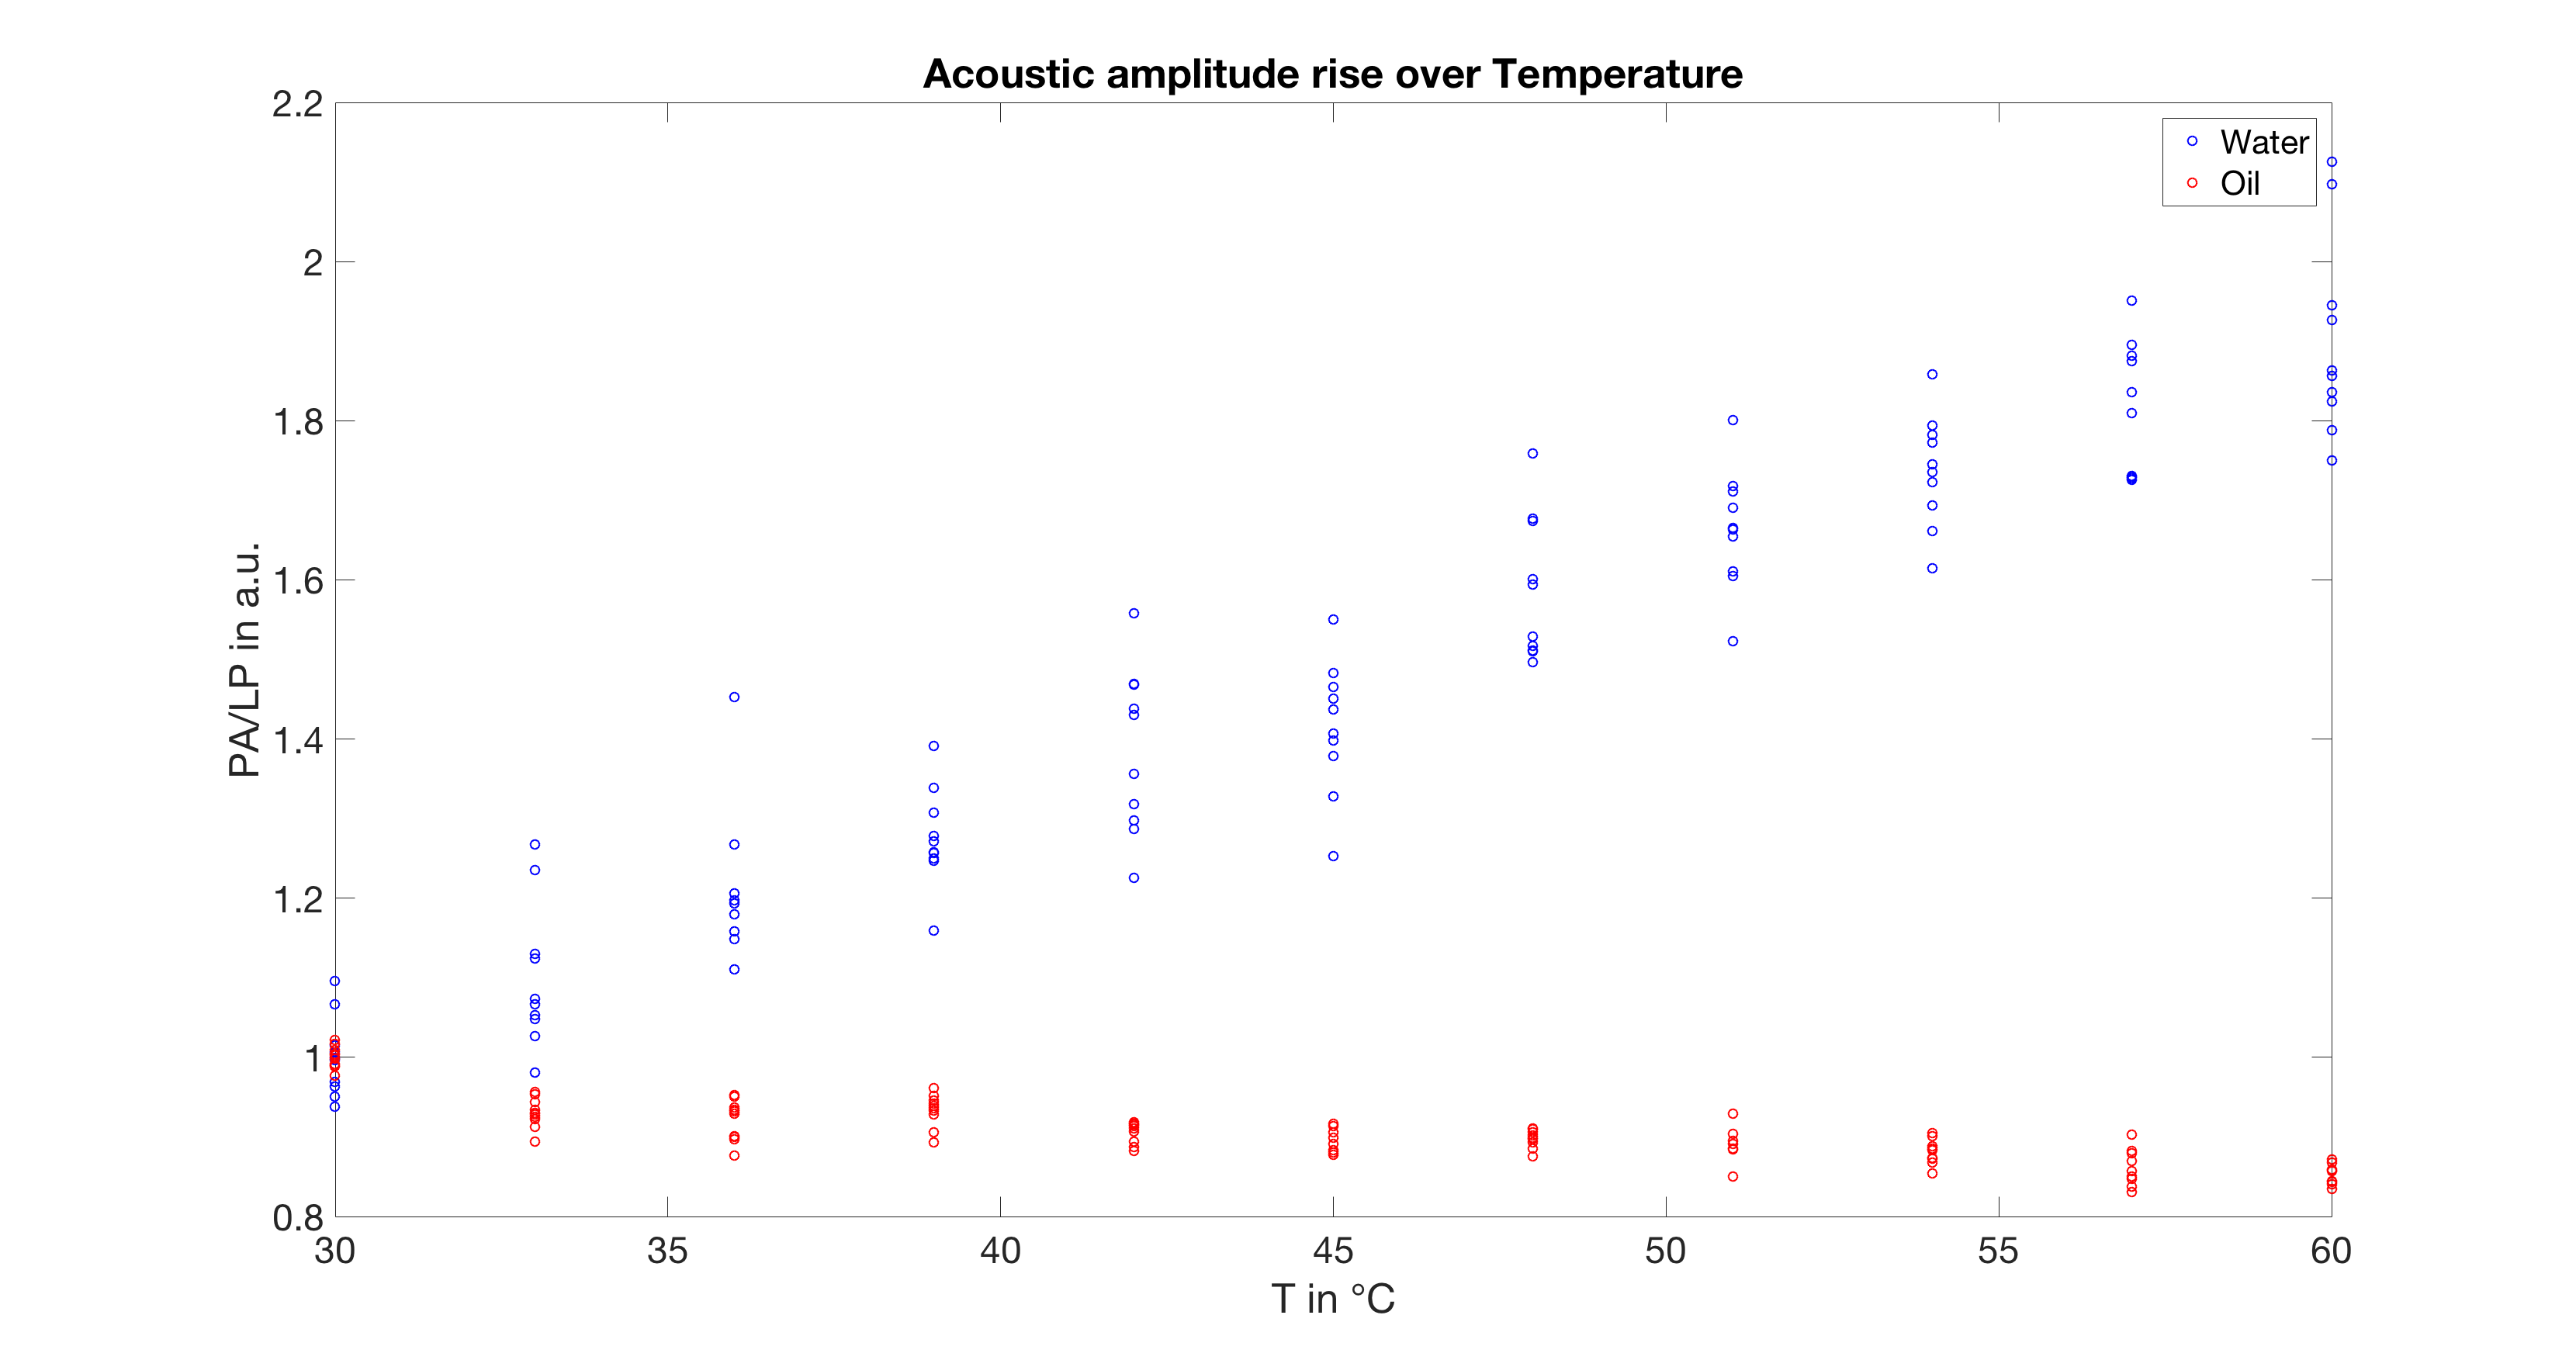
\includegraphics[width = \textwidth, height=0.35\textheight]{04_ex-results_of_PAM/images/GRproof.png}
\end{minipage}
b)
\begin{minipage}{\textwidth}

	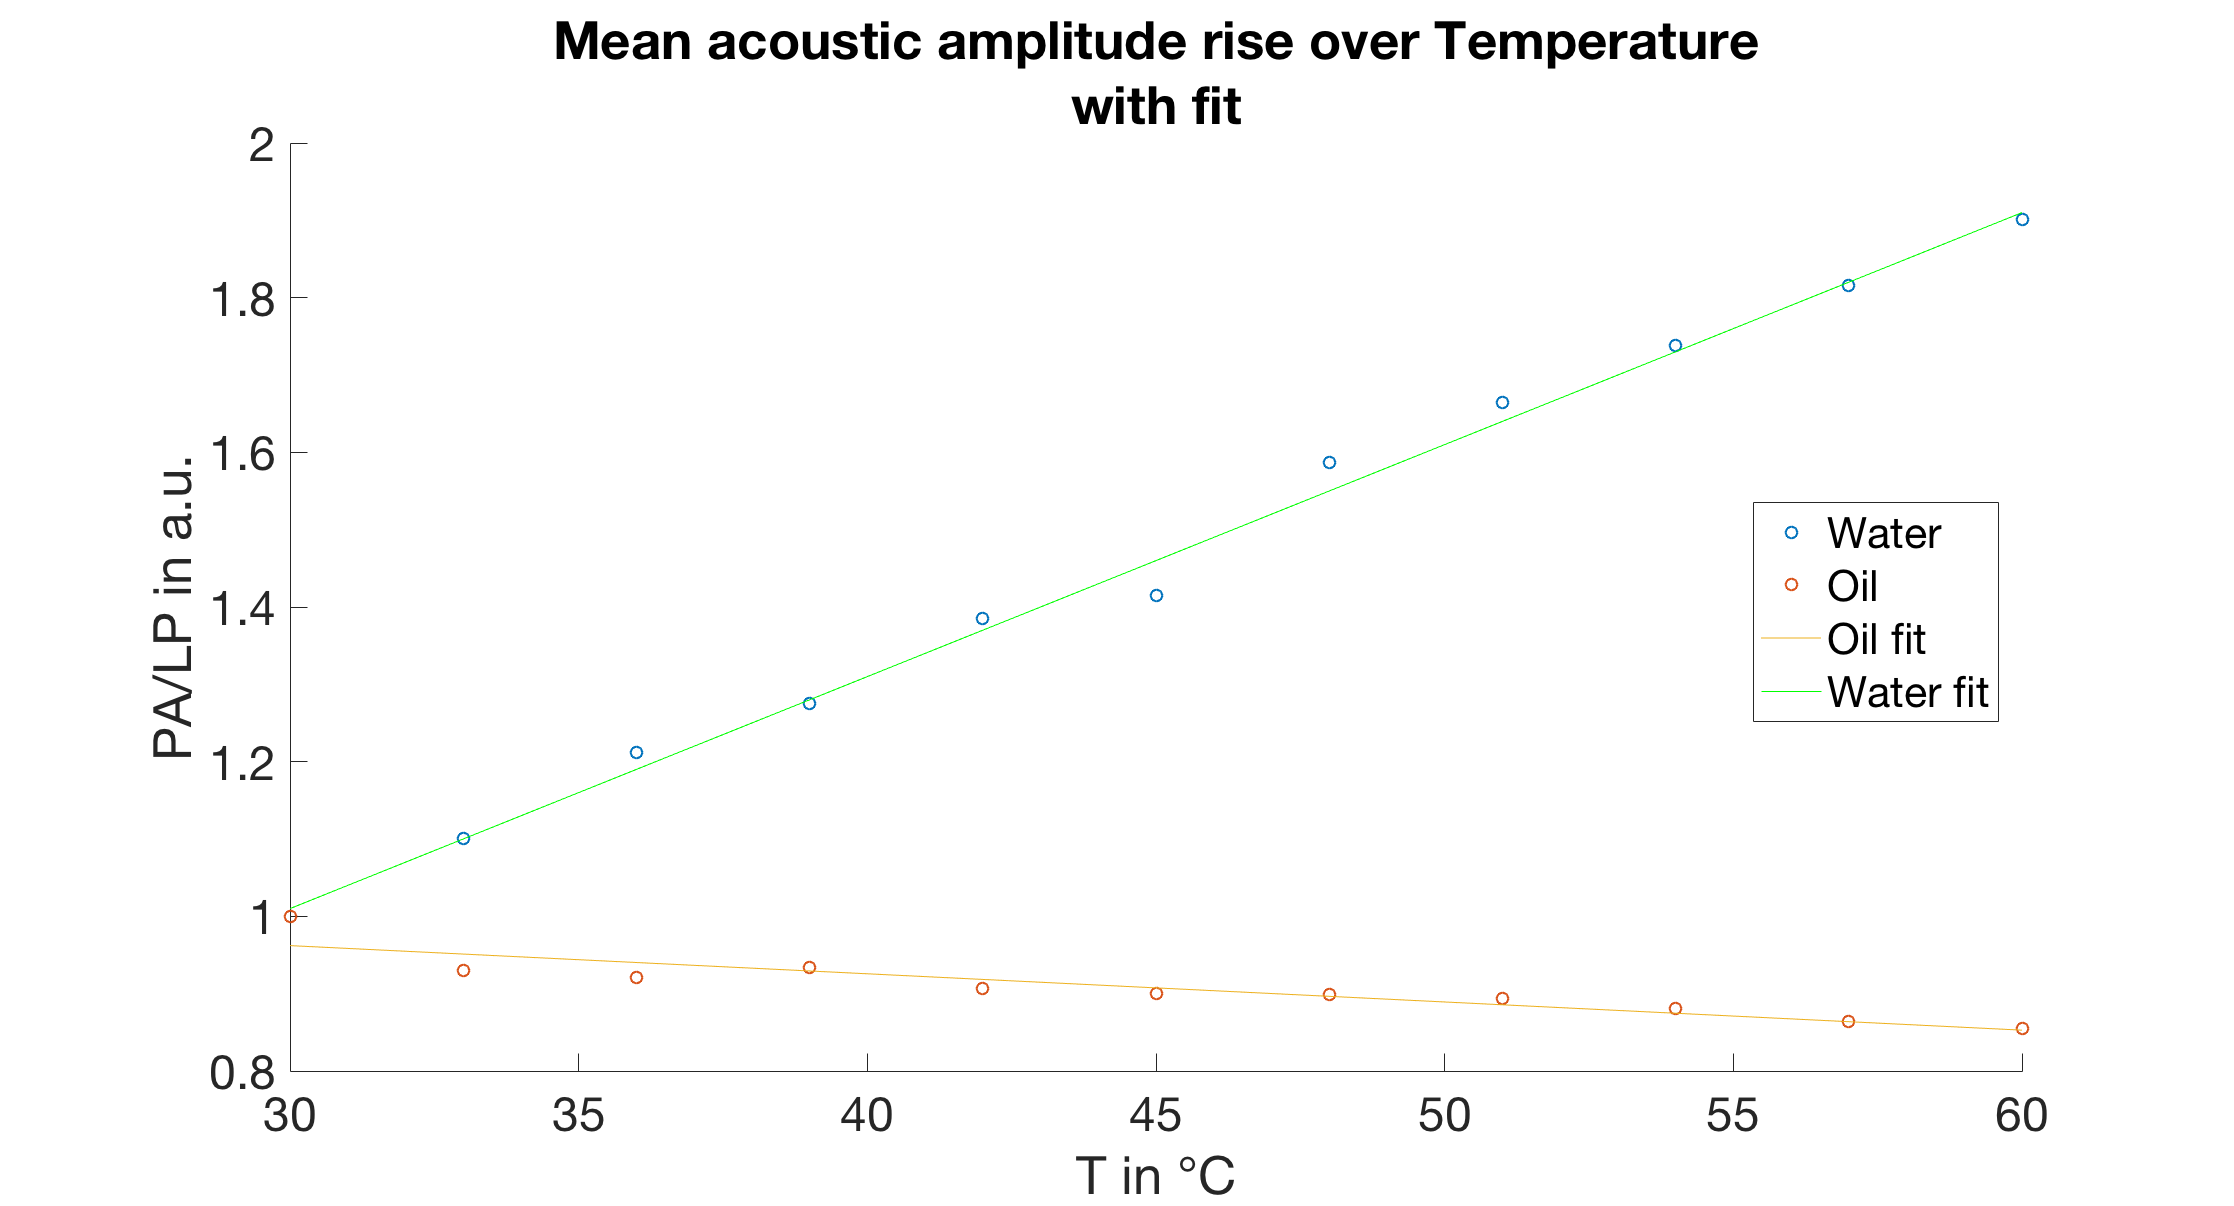
\includegraphics[width = \textwidth, height=0.35\textheight]{04_ex-results_of_PAM/images/meanGRproof.png}
\end{minipage}

\caption{In a) the sampled data for water and oil is displayed and in b) a fit is drawn through the mean values of a). The fit functions are $f_{oil}(T) = -0.0036 \cdot T +1.1$ and $f_{water}(x) = 0.03 \cdot T + 0.11$. The plots in a) and b) are normalized to the mean value at 30~$^\circ C$ and also the photoacoustic amplitudes are normalized to the laser power (LP).}
\label{fig:measuredGRproof}
\end{figure}

In Figure \ref{fig:measuredGRproof} b), it can be seen, that the photoacoustic amplitude for water nearly doubles if the temperature is increased from 30~$^\circ C$ to  60~$^\circ C$, while the effect is weaker for oil and is going in the opposite direction.\\
The photoacoustic amplitudes are normalized to the laser power and the dye is uniformly distributed, so that a constant $\mu_a$ can be assumed. According to equation \ref{eq:p_0}, it can be concluded that the increased (water) or decreased (oil) amplitude is a consequence of a changed $\Gamma$. This leads to a applicable contrast mechanism, here for water and oil, as shown in section \ref{sec:GReffect}.\\
Additional there is to mention that for biological issues, temperatures close to or below 0~$^\circ C$ make no sense to investigate, because of the freezing point of water. But it is crucial not to exceed the boiling point of 100~$^\circ C$. Therefore it is important to keep the laser power for GR-PAM in certain limits to avoid cavitation or ablation, but it has to be strong enough to apply a certain temperature rise. 

\subsection{Experimental results of GR-PAM}

The verified Grueneisen effect were applied to microscopy. Therefore, the used system is described and GR-PAM is compared to OR-PAM. Additionally properties of the used specimen, OrangeG dyed water and paprika powder stained rizinus oil, are determined.

\subsubsection{GR-PAM laser setup}

In order to employ two laser pulses for GR-PAM to the system several setups are possible. By virtue of needing a time delay between the pulses in the $\mu s$ range the laser systems available (All of them have a 10kHz repetition rate) are to slow to use a single one. Therefore a two laser system were built.\\
As basis the OR-PAM setup (introduced in section \ref{sec:ORPAMsetup}) were used and reamed with the part inside the dashed box in figure \ref{fig:GRPAMsetup}. In a first setup version the chosen Laser B was a cw-laser from Spectra-Physics (Excelsior-532-100, $\lambda$ = 532~$nm$) and B* were a liquid crystal retarder (Thorlabs LCC 1233-A). This element changes the polarization of incoming light due to the applied voltage. The control unit of the LCC allows to save two voltage values that can be toggled due to an external trigger. If one value is chosen in a way, that there is the maximum laser power after the beam splitter (BS) and the other one with non, it can be used as a switch for the cw-laser beam. 

\begin{figure}[H]
	\centering
	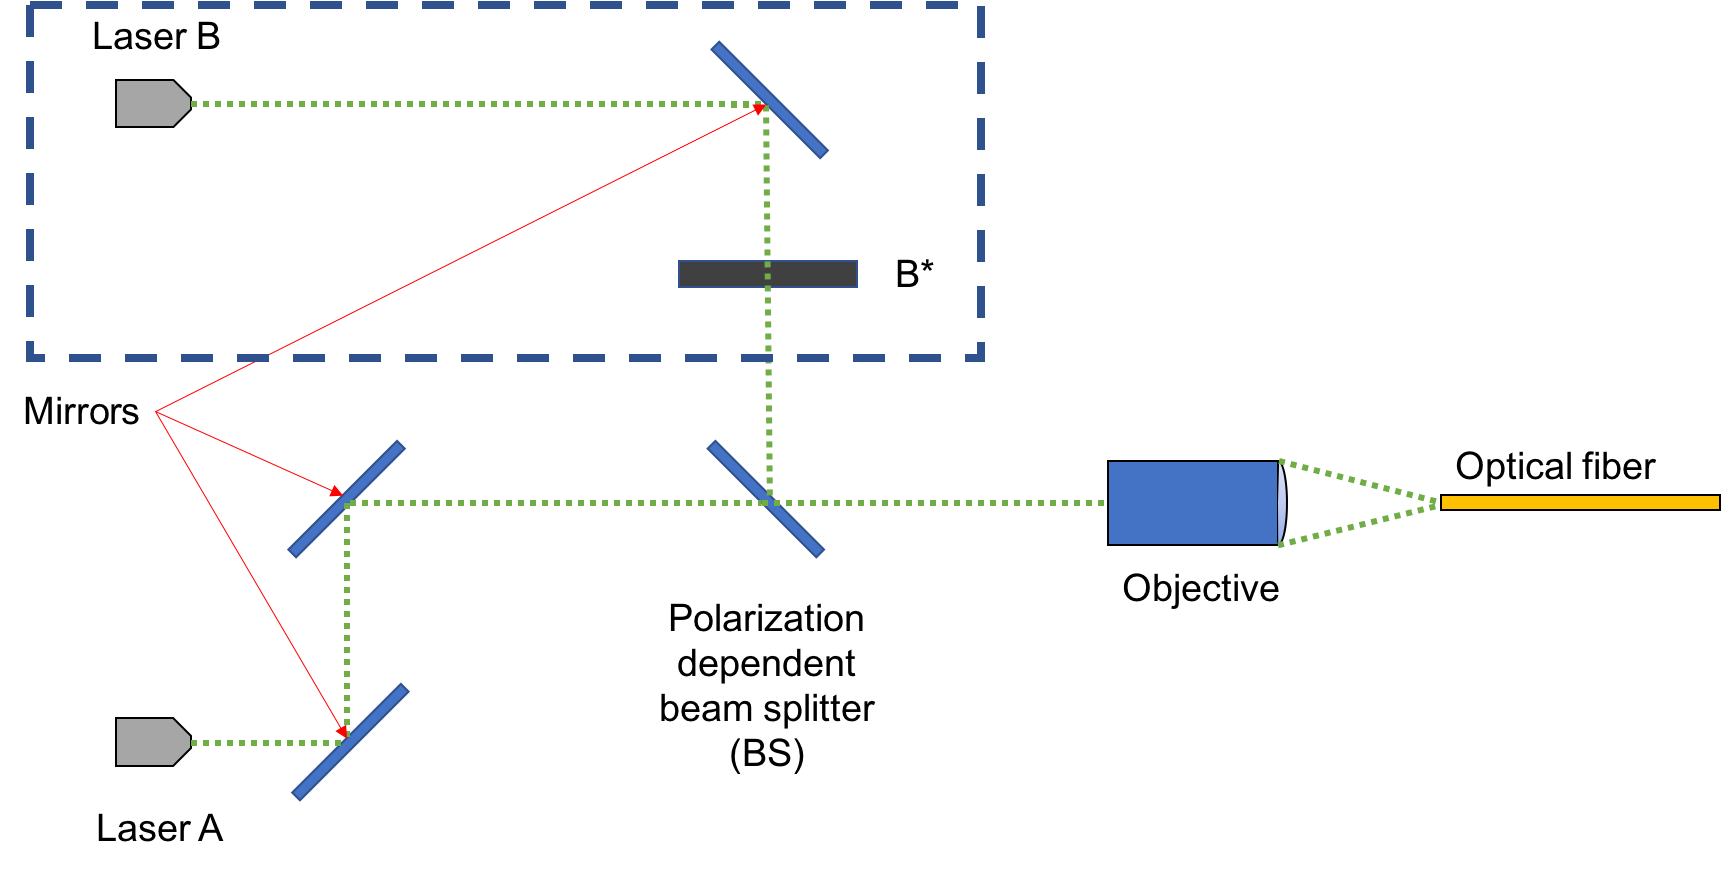
\includegraphics[ height=0.35\textheight]{04_ex-results_of_PAM/images/GR_PAMsetup.png}
	\caption{Illustrated GR-PAM setup. The part inside the dashed box is the part added to the OR-PAM setup to do GR-PAM. Laser A is a LCM-DTL-319QT with $\lambda$ = 527$nm$.}
	\label{fig:GRPAMsetup}
\end{figure}

The disadvantage of this configuration is that the LCC has a rise time $t_r$ of about 500~$\mu s$ and a fall time $t_f$ of 25~$ms$. This leads to a slow scan velocity. \\
In order to increase the scan speed, the dashed part were replaced and only the deflection mirror remains. Laser B were substituted by a pulsed laser (Innolas mosquitoo $\lambda$ = 532~$nm$) and B* with a wave plate that is mounted on a rotary mount. This allows a tuning of the laser power of Laser B that is coupled into the optical fiber. Thus both lasers have a repetition rate of 10~$kHz$, the limiting factor is the maximum possible scan speed the linear stages and scanhead can move. \\
The triggering of the lasers and therefore the delay time between the pulses were generated by the Delay Generator mentioned before.

\subsubsection{Absorption coefficient of OrangeG and colored rizinus oil}
\label{sec:oGrizOilabsoption}
As shown in figure \ref{fig:GRPAMsetup} the two used laser systems, for the GR-PAM measurements, have differing wavelengths. In most cases the absorption difference is negligible, meaning case 1) in section \ref{sec:dualPulseTechnique} is valid. But in some cases option 2) or 3) emerge.\\
However, in Figure \ref{fig:orangeGricinus} the absorption coefficient for OrangeG and, as a reference, the also used paprika powder colored rizinus oil is shown. The OrangeG were dissolved in water with a concentration of 10~$g/l$. The concentration of paprika dye in the oil is unknown. 

\begin{figure}[H]
	\centering
	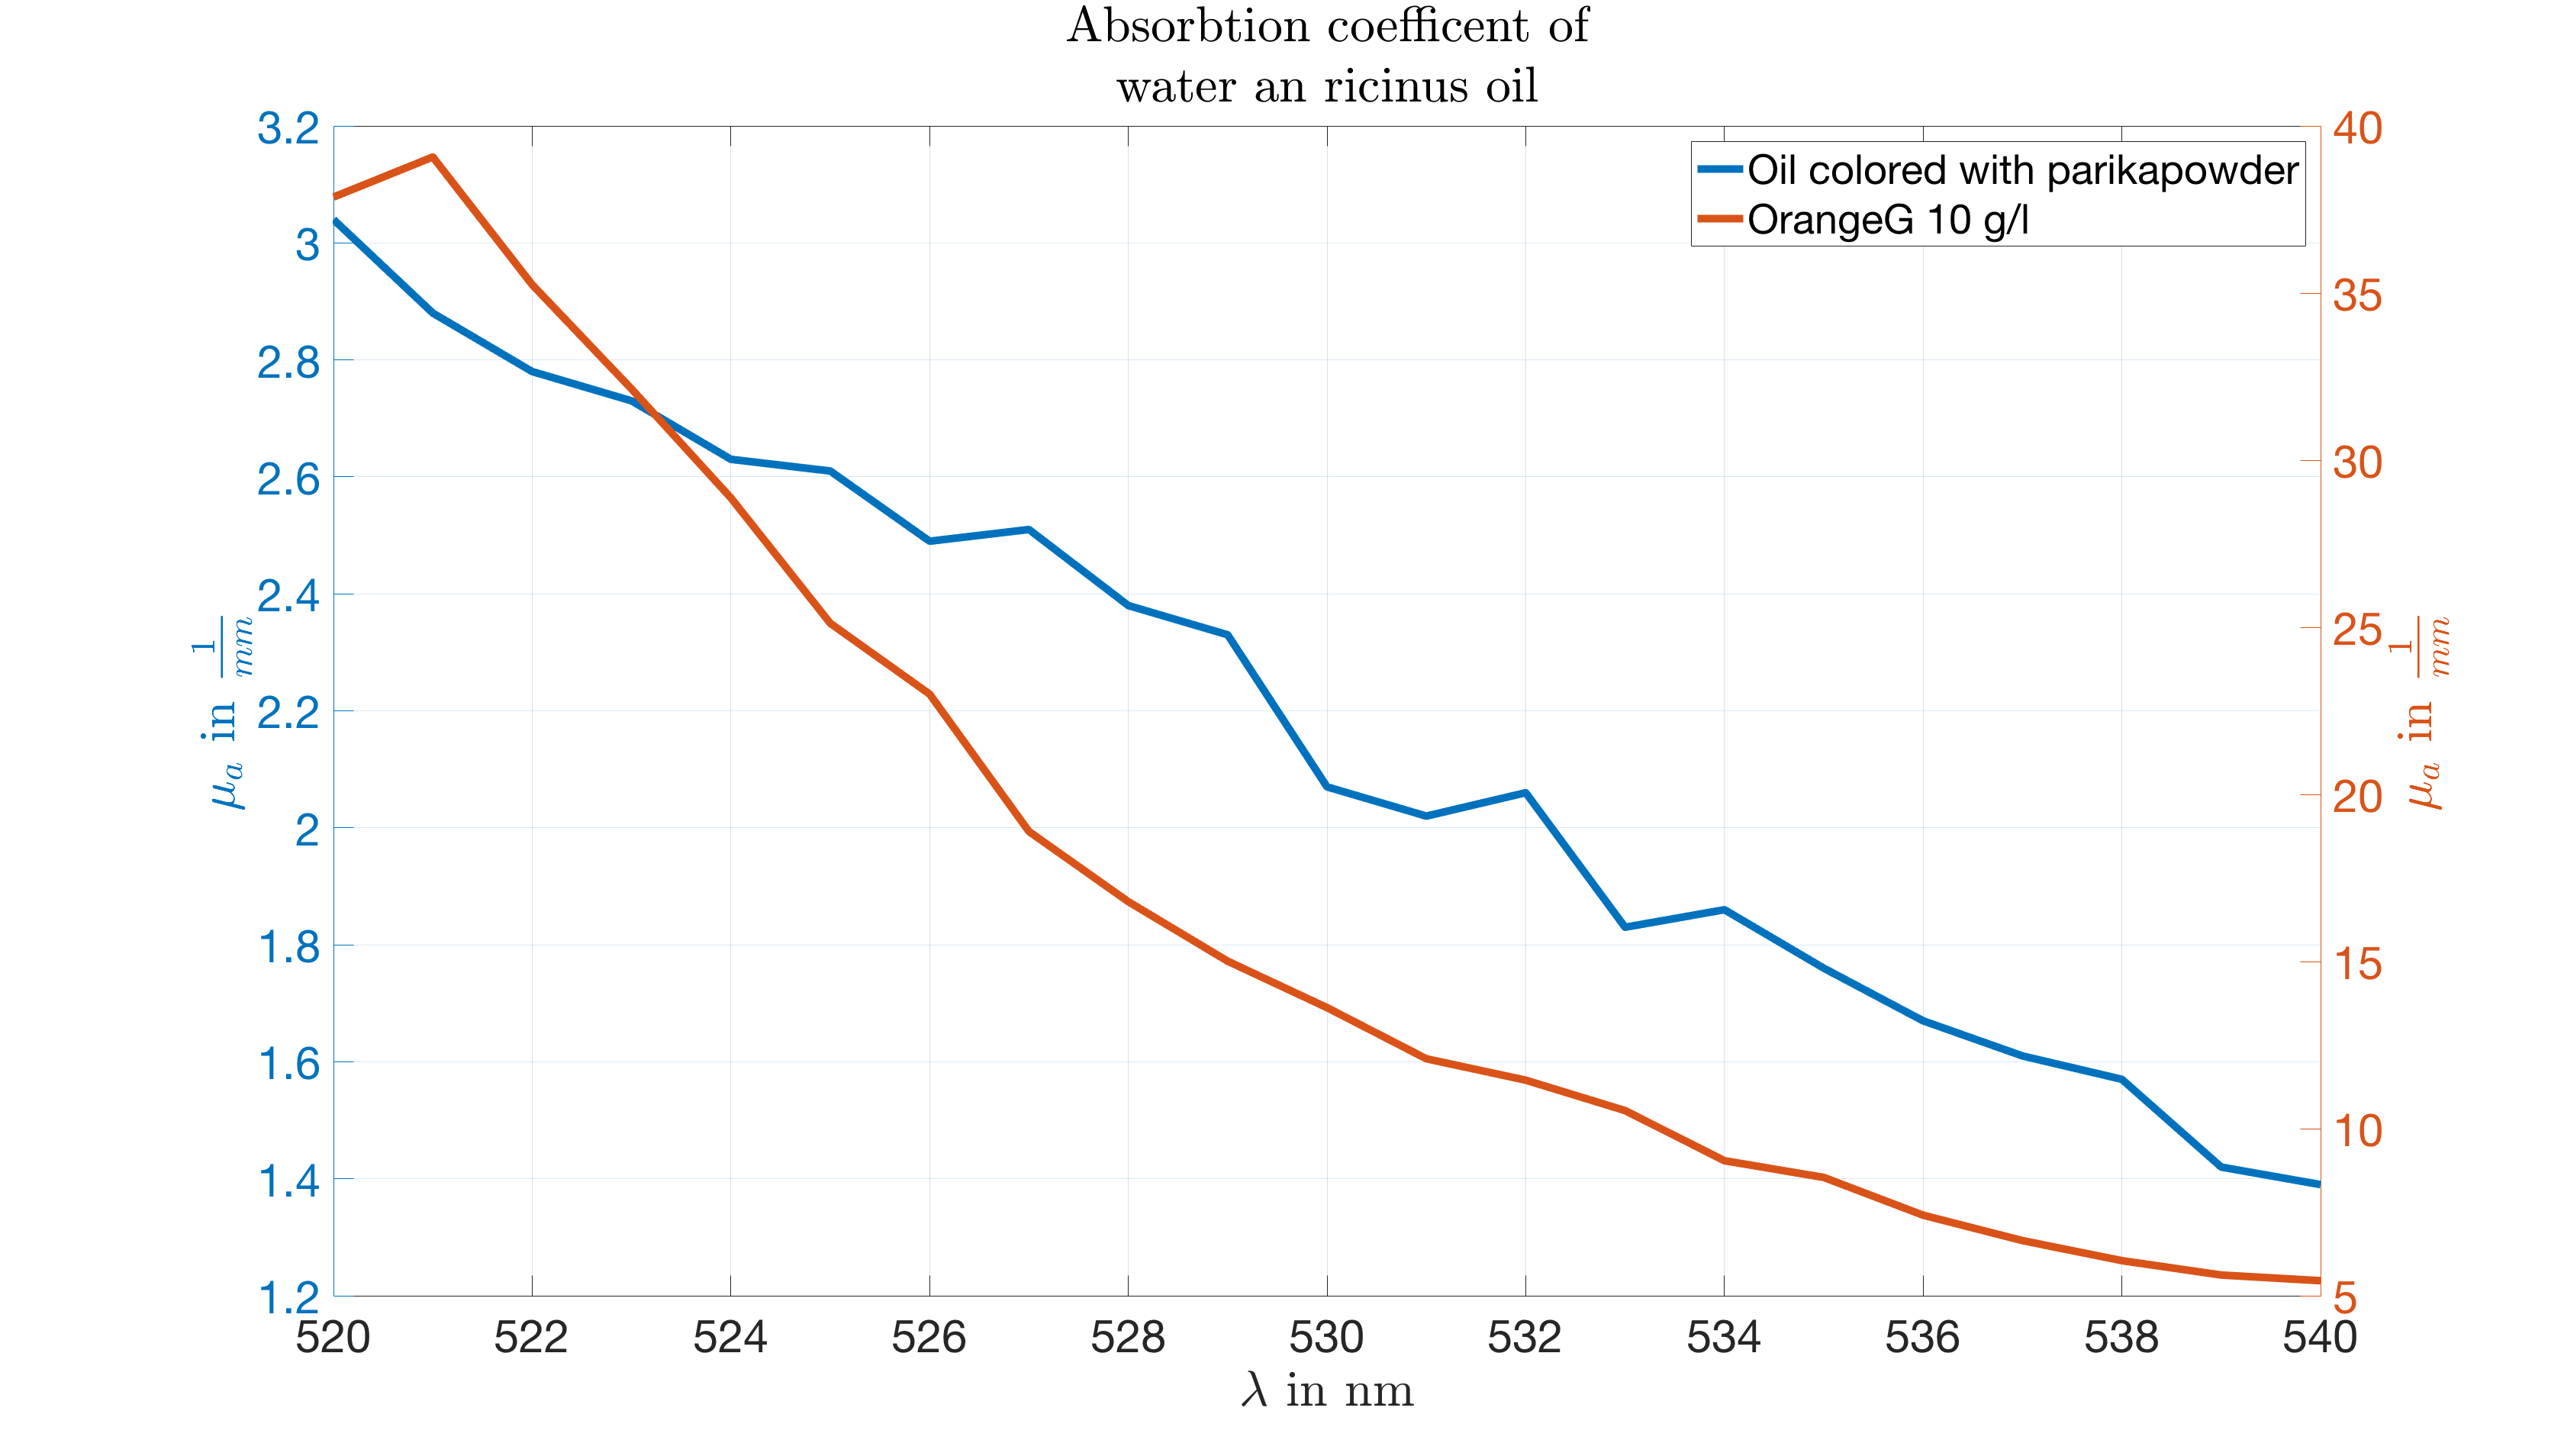
\includegraphics[ height=0.35\textheight]{04_ex-results_of_PAM/images/orangeGricinusMu_a.png}
	\caption{Absorption coefficient of OrangeG dissolved in water and ricinus oil colored with paprika powder, in a wavelength range of 520~$nm$ to 540~$nm$.}
	\label{fig:orangeGricinus}
\end{figure}

It can be seen that there is a difference between the absorption coefficient values for the used wavelengths (527~$nm$ and 532~$nm$). This results for the rizinus oil $\Delta\mu_a$ = 0.45~$\frac{1}{mm}$ and $\Delta\mu_a$  = 7.44~$\frac{1}{mm}$ for OrangeG.\\
Therefore, it is to be considered that the measurements, there OrangeG were used, are done with configuration two. Thus the 532~$nm$ laser were used to operate the heating pulse and the 527~$nm$ laser the detection pulse.

\subsubsection{Comparison between OR-PAM and GR-PAM}
\label{sec:ORGRcomp}

In order to compare OR-PAM with GR-PAM a small container were filled with OrangeG colored water and a droplet of paprika powder colored rizinus oil were deposited. In respect of the results of section \ref{sec:oGrizOilabsoption} the 532$nm$ laser were chosen to apply the heating pulse and the 527$nm$ the detection pulse. Figure \ref{fig:imgGRproof} shows the taken image. 

\begin{figure}[H]
	a)
	\begin{minipage}{\textwidth}
		\centering	
		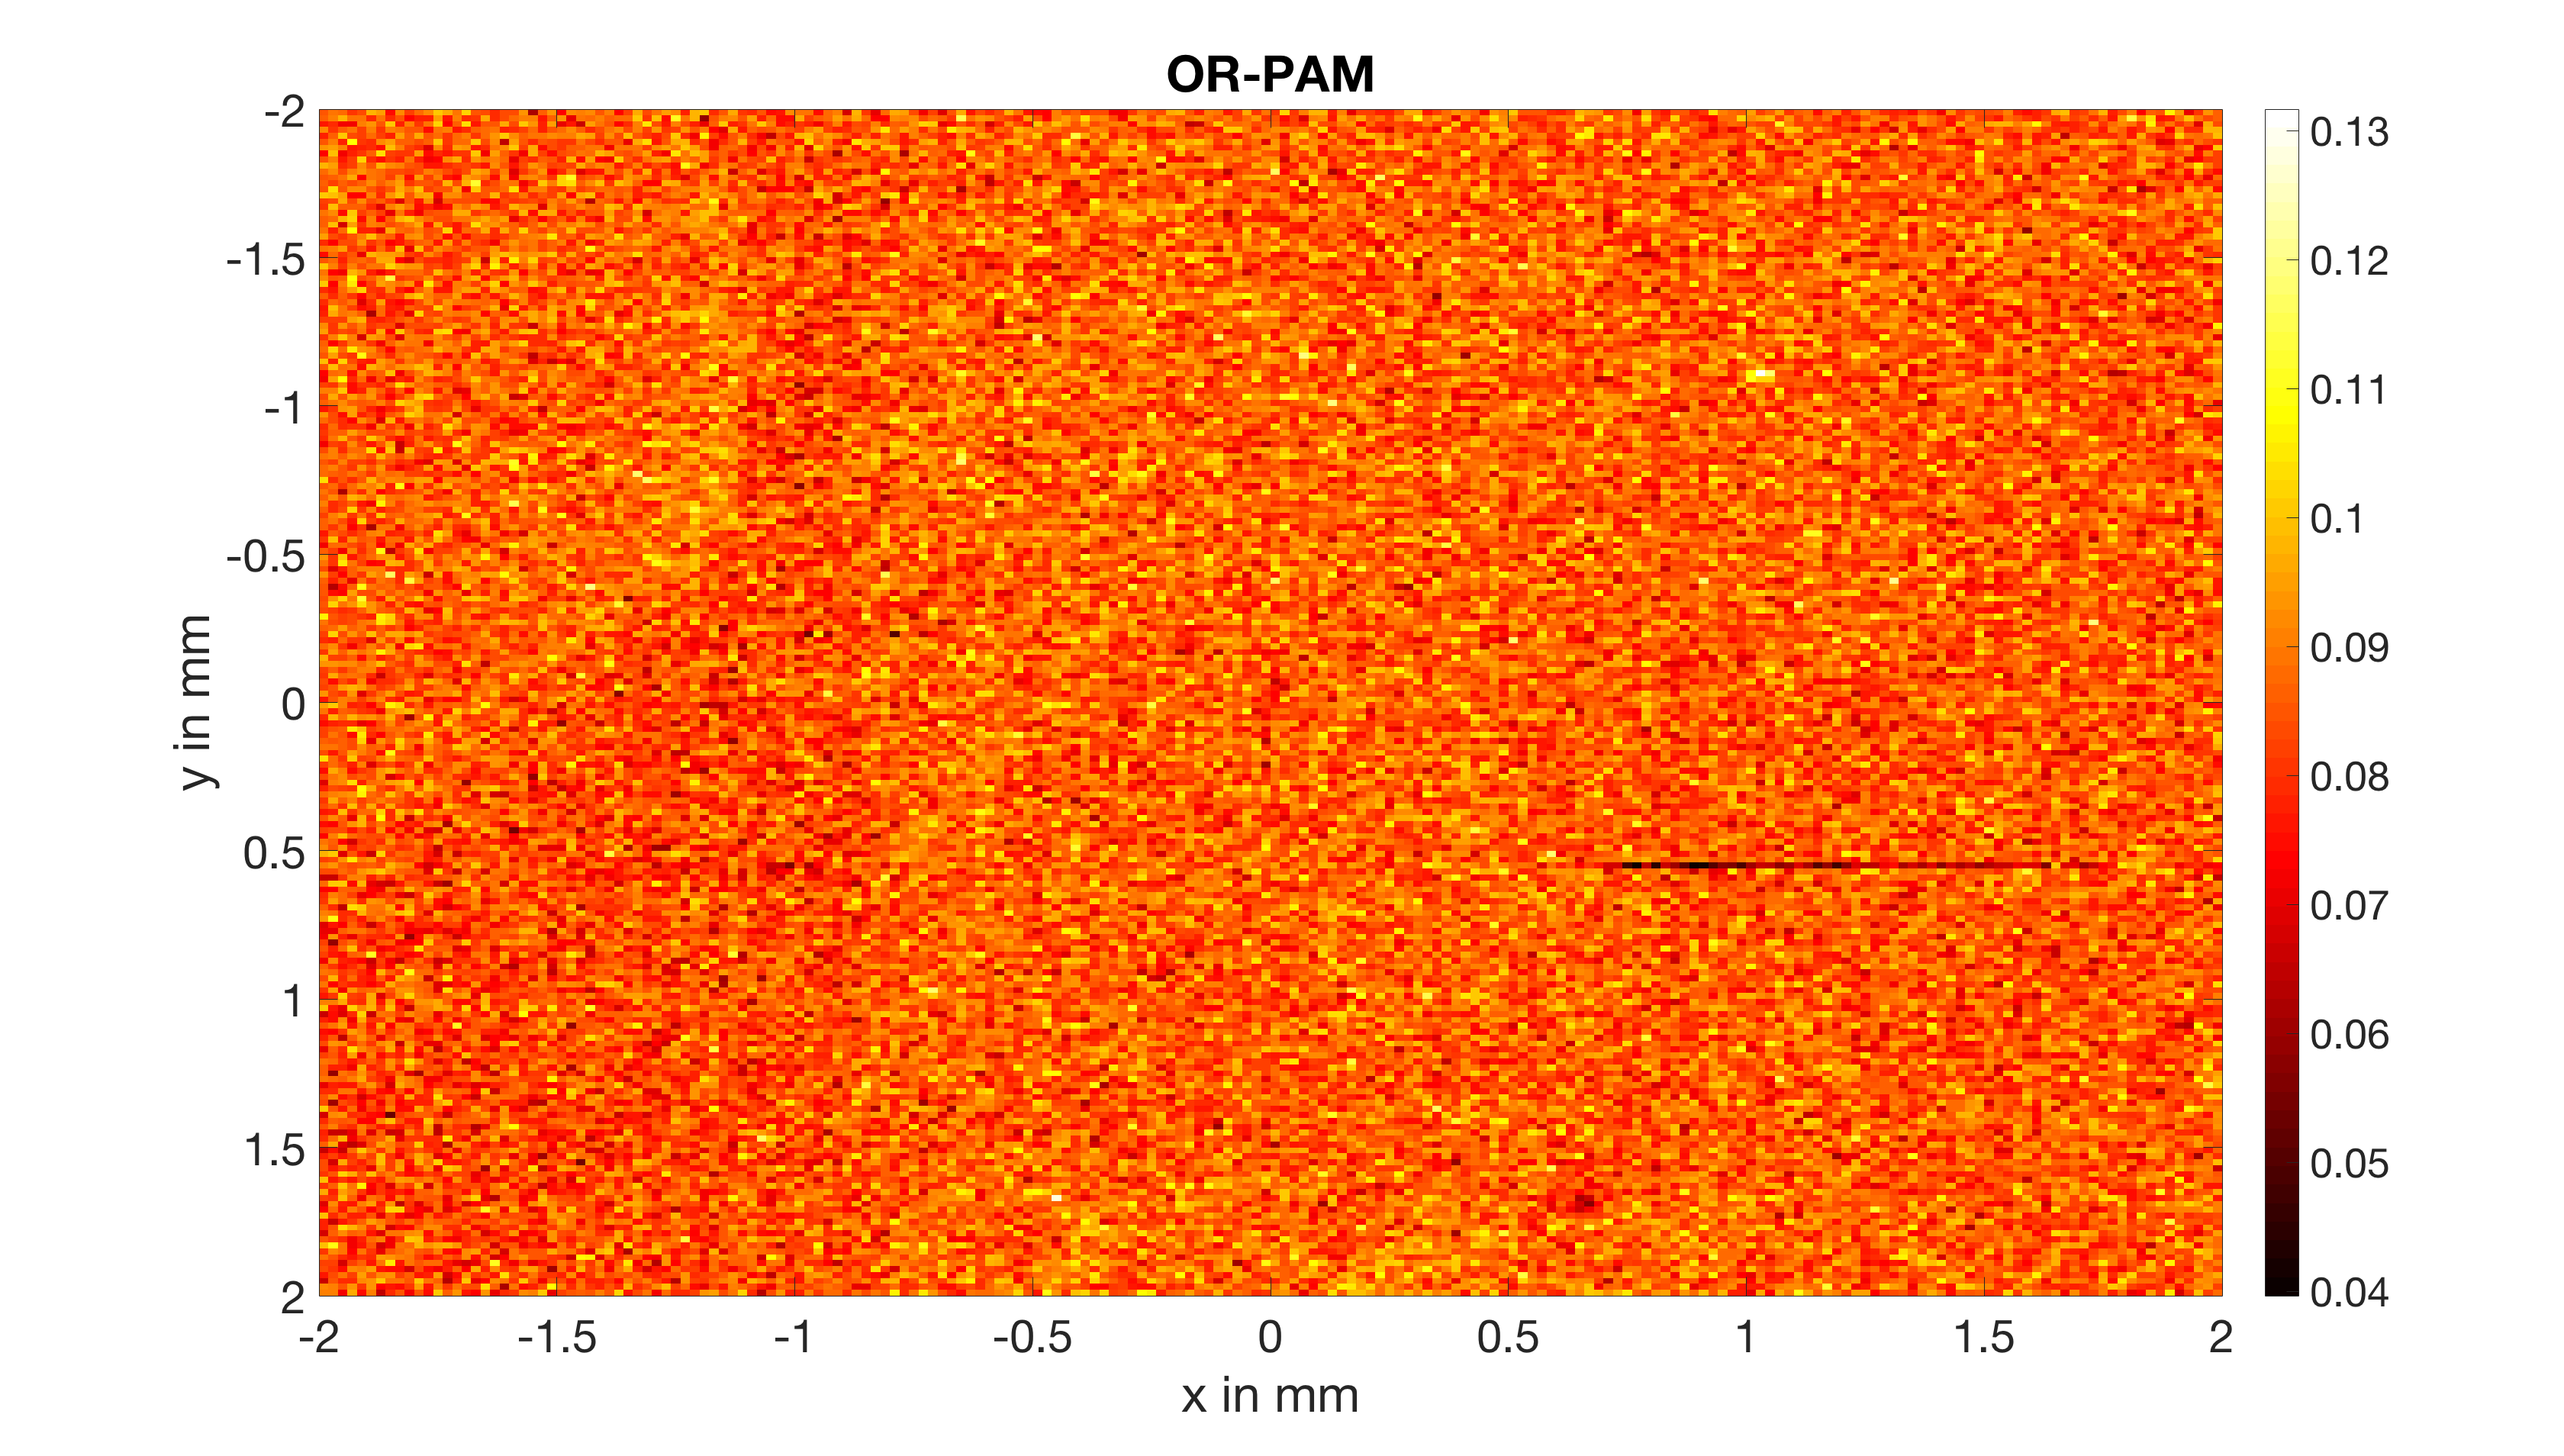
\includegraphics[width = 0.8\textwidth, height=0.38\textheight]{04_ex-results_of_PAM/images/oilDrop_OR.png}
	\end{minipage}	
	b)
	\begin{minipage}{\textwidth}
		\centering	
		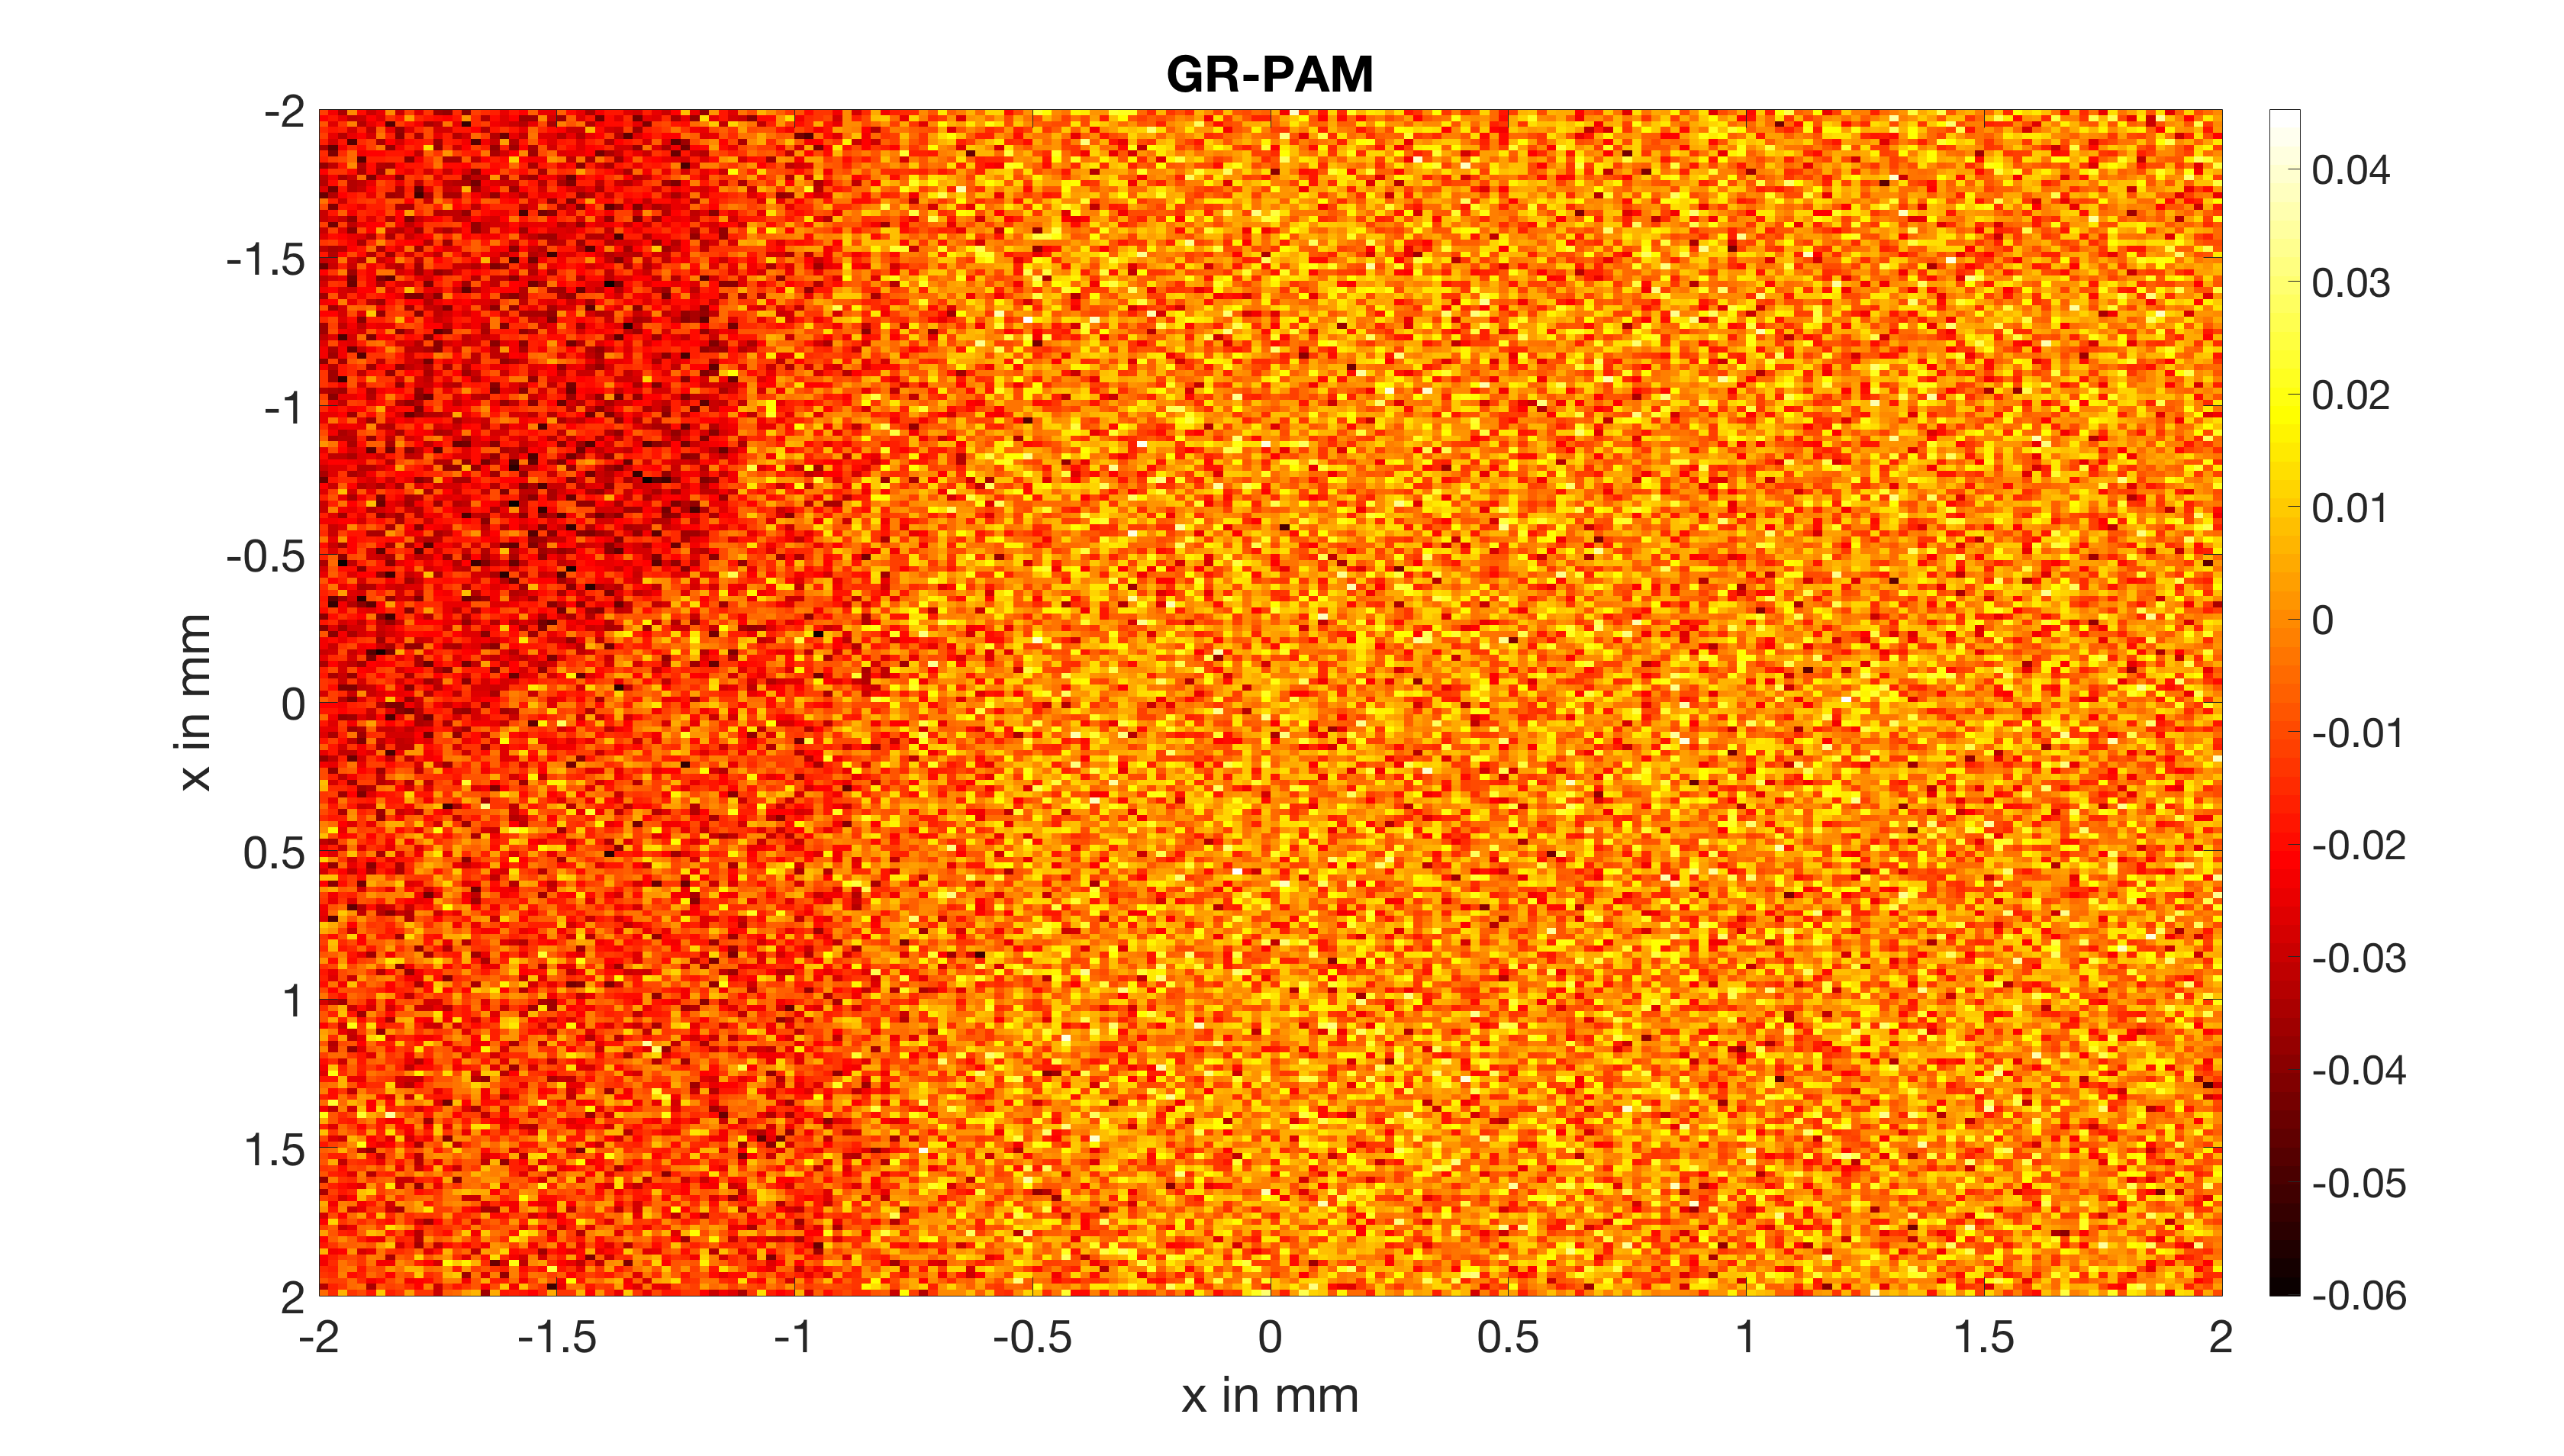
\includegraphics[width = 0.8\textwidth, height=0.38\textheight]{04_ex-results_of_PAM/images/oilDrop_GR.png}
	\end{minipage}
	
	\caption{Image of a rizinus oil droplet in a OrangeG reservoir. The scan area is 4 x 4~$mm$ with 200 points and a step size of 20~$\mu m$ taken in each direction.}
	\label{fig:imgGRproof}
\end{figure}

The oil droplet is placed in the upper left corner of the container. \\
Figure \ref{fig:imgGRproof} a) shows the OR-PAM image, there just the slight differences in the absorption coefficient are visible. The OR-PAM information is taken from the photoacoustic amplitude generated by the first laser pulse. Whereas figure \ref{fig:imgGRproof} b) shows the contrast between the positive Grueneisen effect for the OrangeG colored water and the negative for the rizinus oil.\\
It is important to mention, that the evaluation program takes the maximum amplitude of each data vector, the heating pulse as well as the detection pulse vector. Assuming that the whole two vectors are subtracted from each other, to generate the GR-PAM information, a slight time difference between the peaks results in a wrong representation of the effect.\\
For figure \ref{fig:imgGRblackleaf} a black plastic leaf is imaged.\\

\begin{figure}[H]
	a)
	\begin{minipage}{\textwidth}
		\centering		
		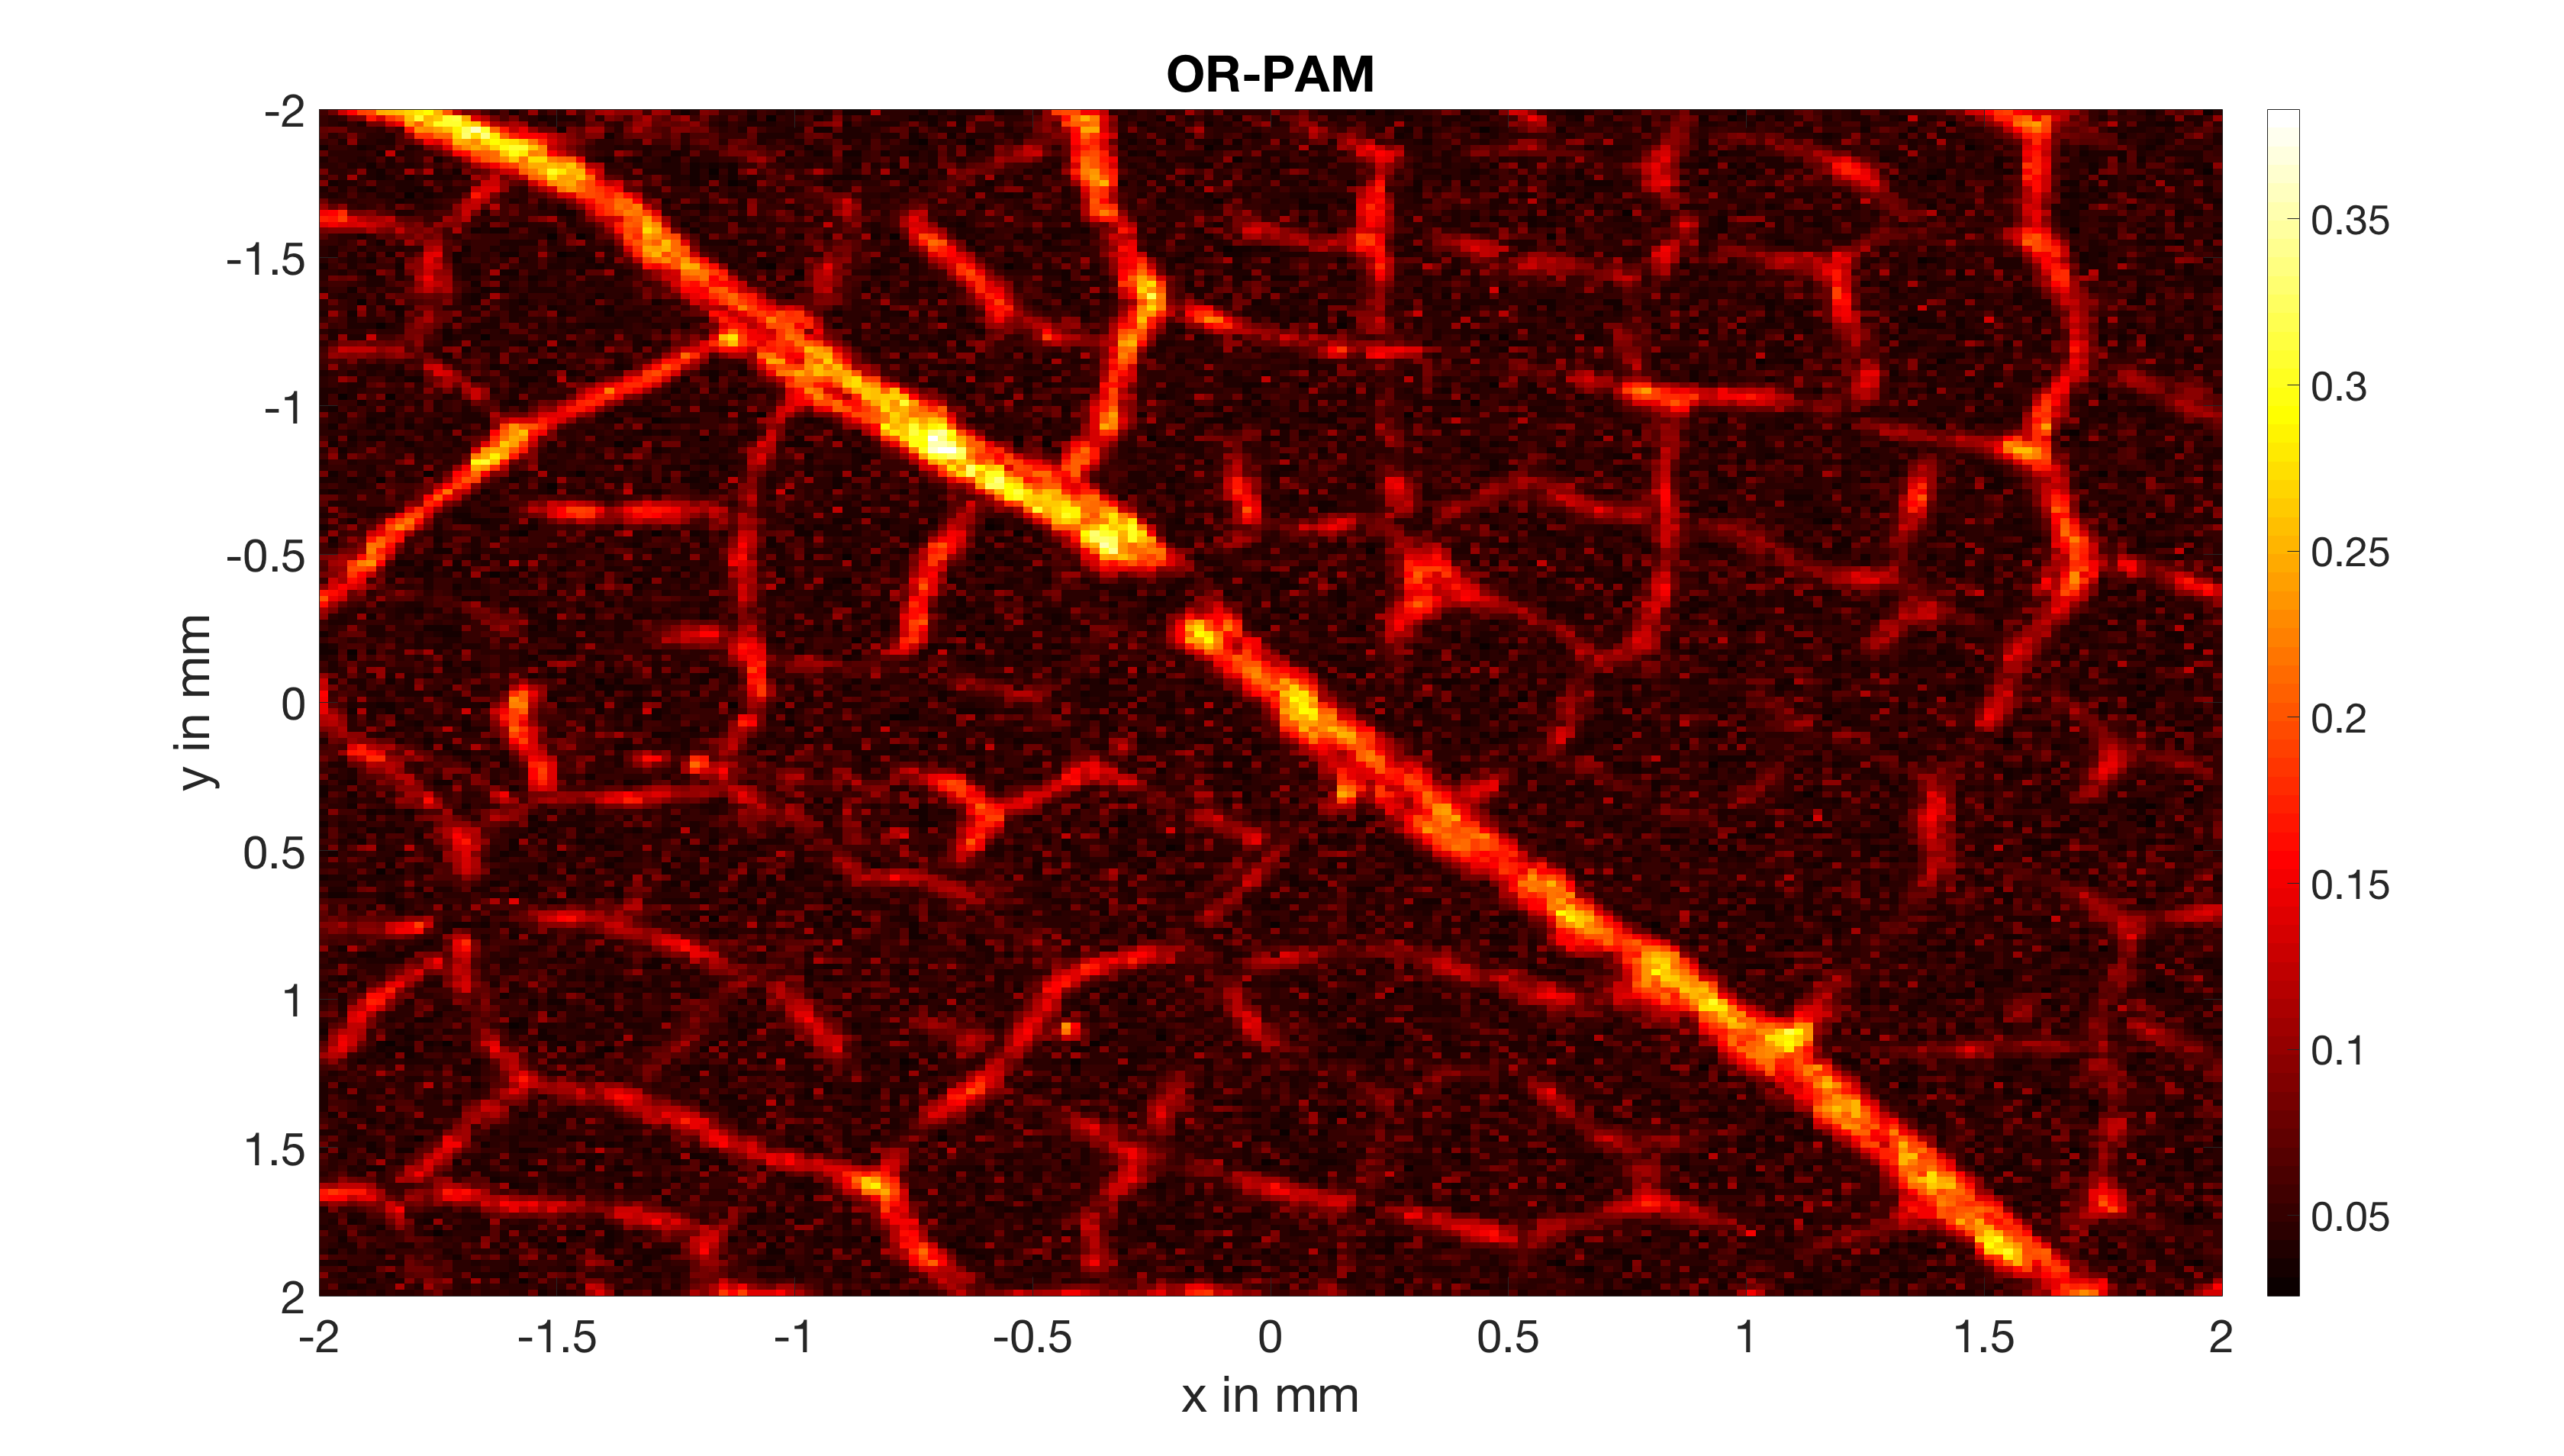
\includegraphics[width = 0.8\textwidth, height=0.38\textheight]{04_ex-results_of_PAM/images/blackleaf_OR.png}
	\end{minipage}	
	b)
	\begin{minipage}{\textwidth}
		\centering		
		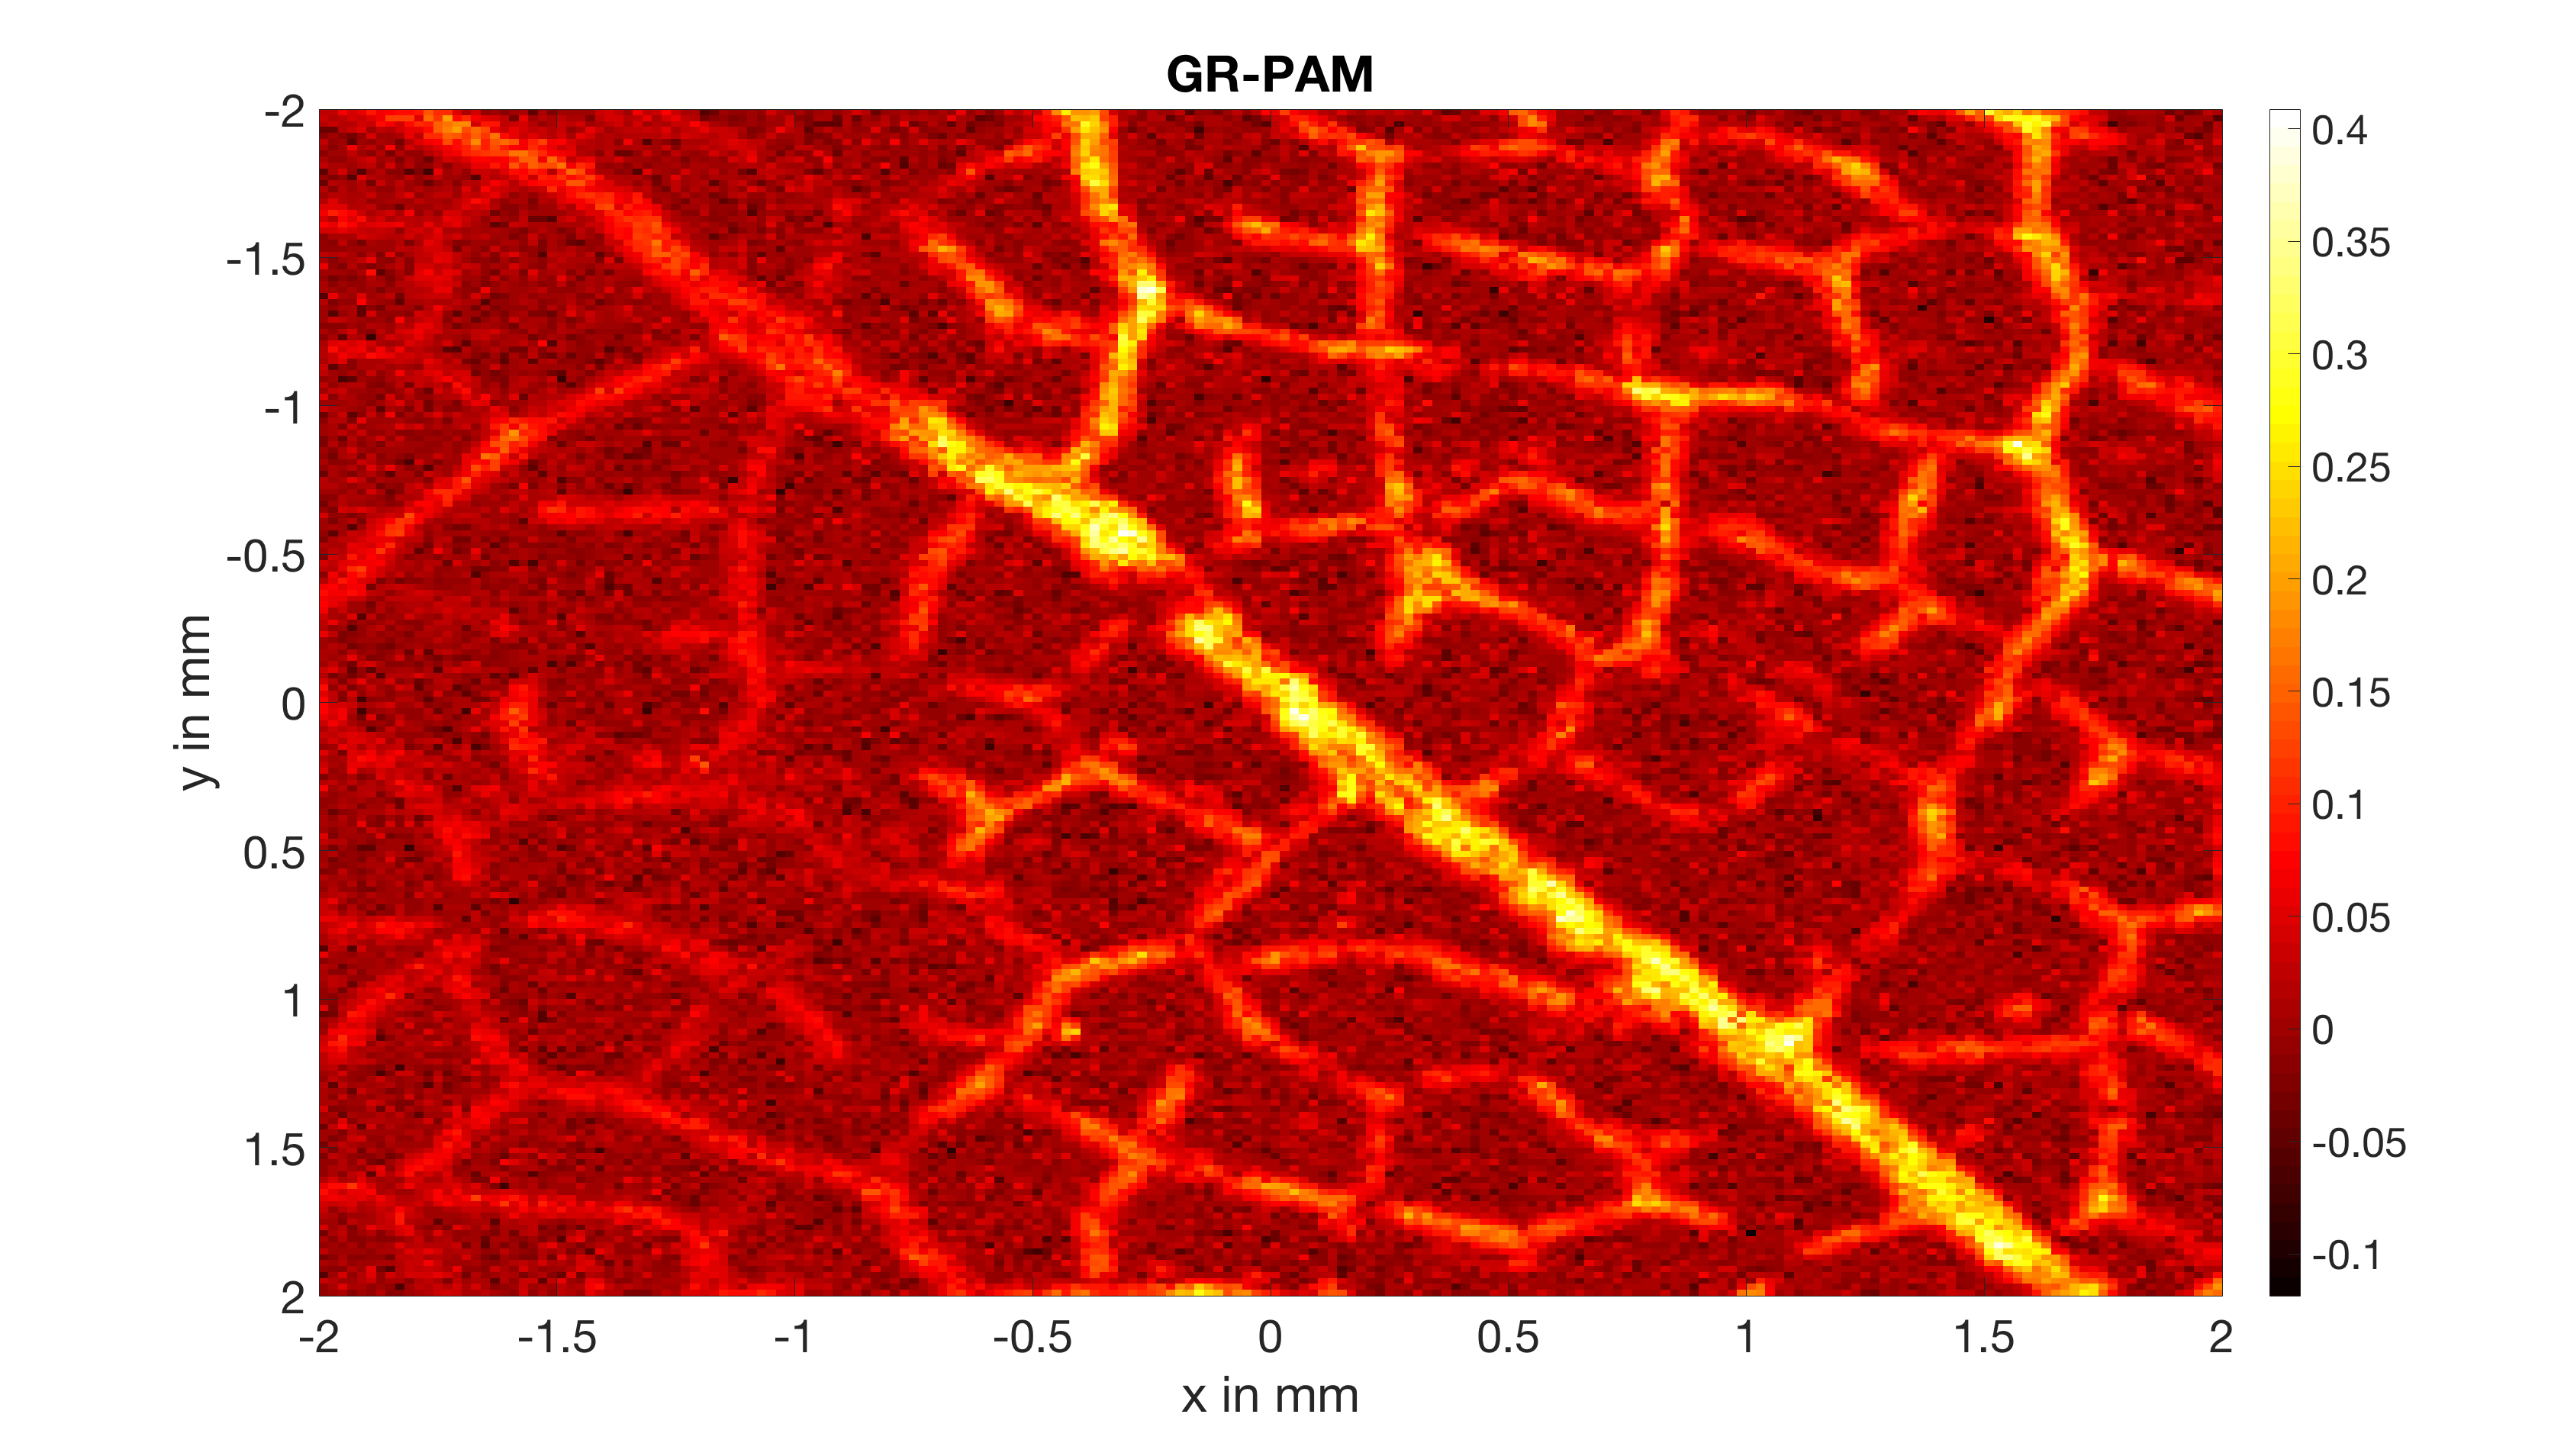
\includegraphics[width = 0.8\textwidth, height=0.38\textheight]{04_ex-results_of_PAM/images/blackleaf_GR.png}
	\end{minipage}
	
	\caption{Image of a black plastic leaf. The scan area is 4 x 4~$mm$ with 200 points and a step size of 20~$\mu m$ taken in each direction.}
	\label{fig:imgGRblackleaf}
\end{figure}

In figure \ref{fig:imgGRblackleaf} a) a conventional OR-PAM picture is shown. Furthermore, \ref{fig:imgGRblackleaf} b) shows a GR-PAM image. It is visible, that in \ref{fig:imgGRblackleaf} b), the left part and some of the ramification is weaker than the others, whereas the main strand appears mostly exceedingly. This can be assigned towards the sectioning capabilities of GR-PAM. 

\subsubsection{Lateral resolution determination}

To determine the resolution of the photoacoustic measurements a resolution target (Edmund Optics, USAF 1951) were scanned. \\
The resolution of an optical system can be found by scanning over a sharp edge, giving a edge spread function (ESF). The derivation of the ESF produces a Gaussian shaped function. Thereby the FWHM can be built, which results the resolution.\\

 \begin{figure}[H]
 	a)
 	\begin{minipage}{0.5\textwidth}		
 		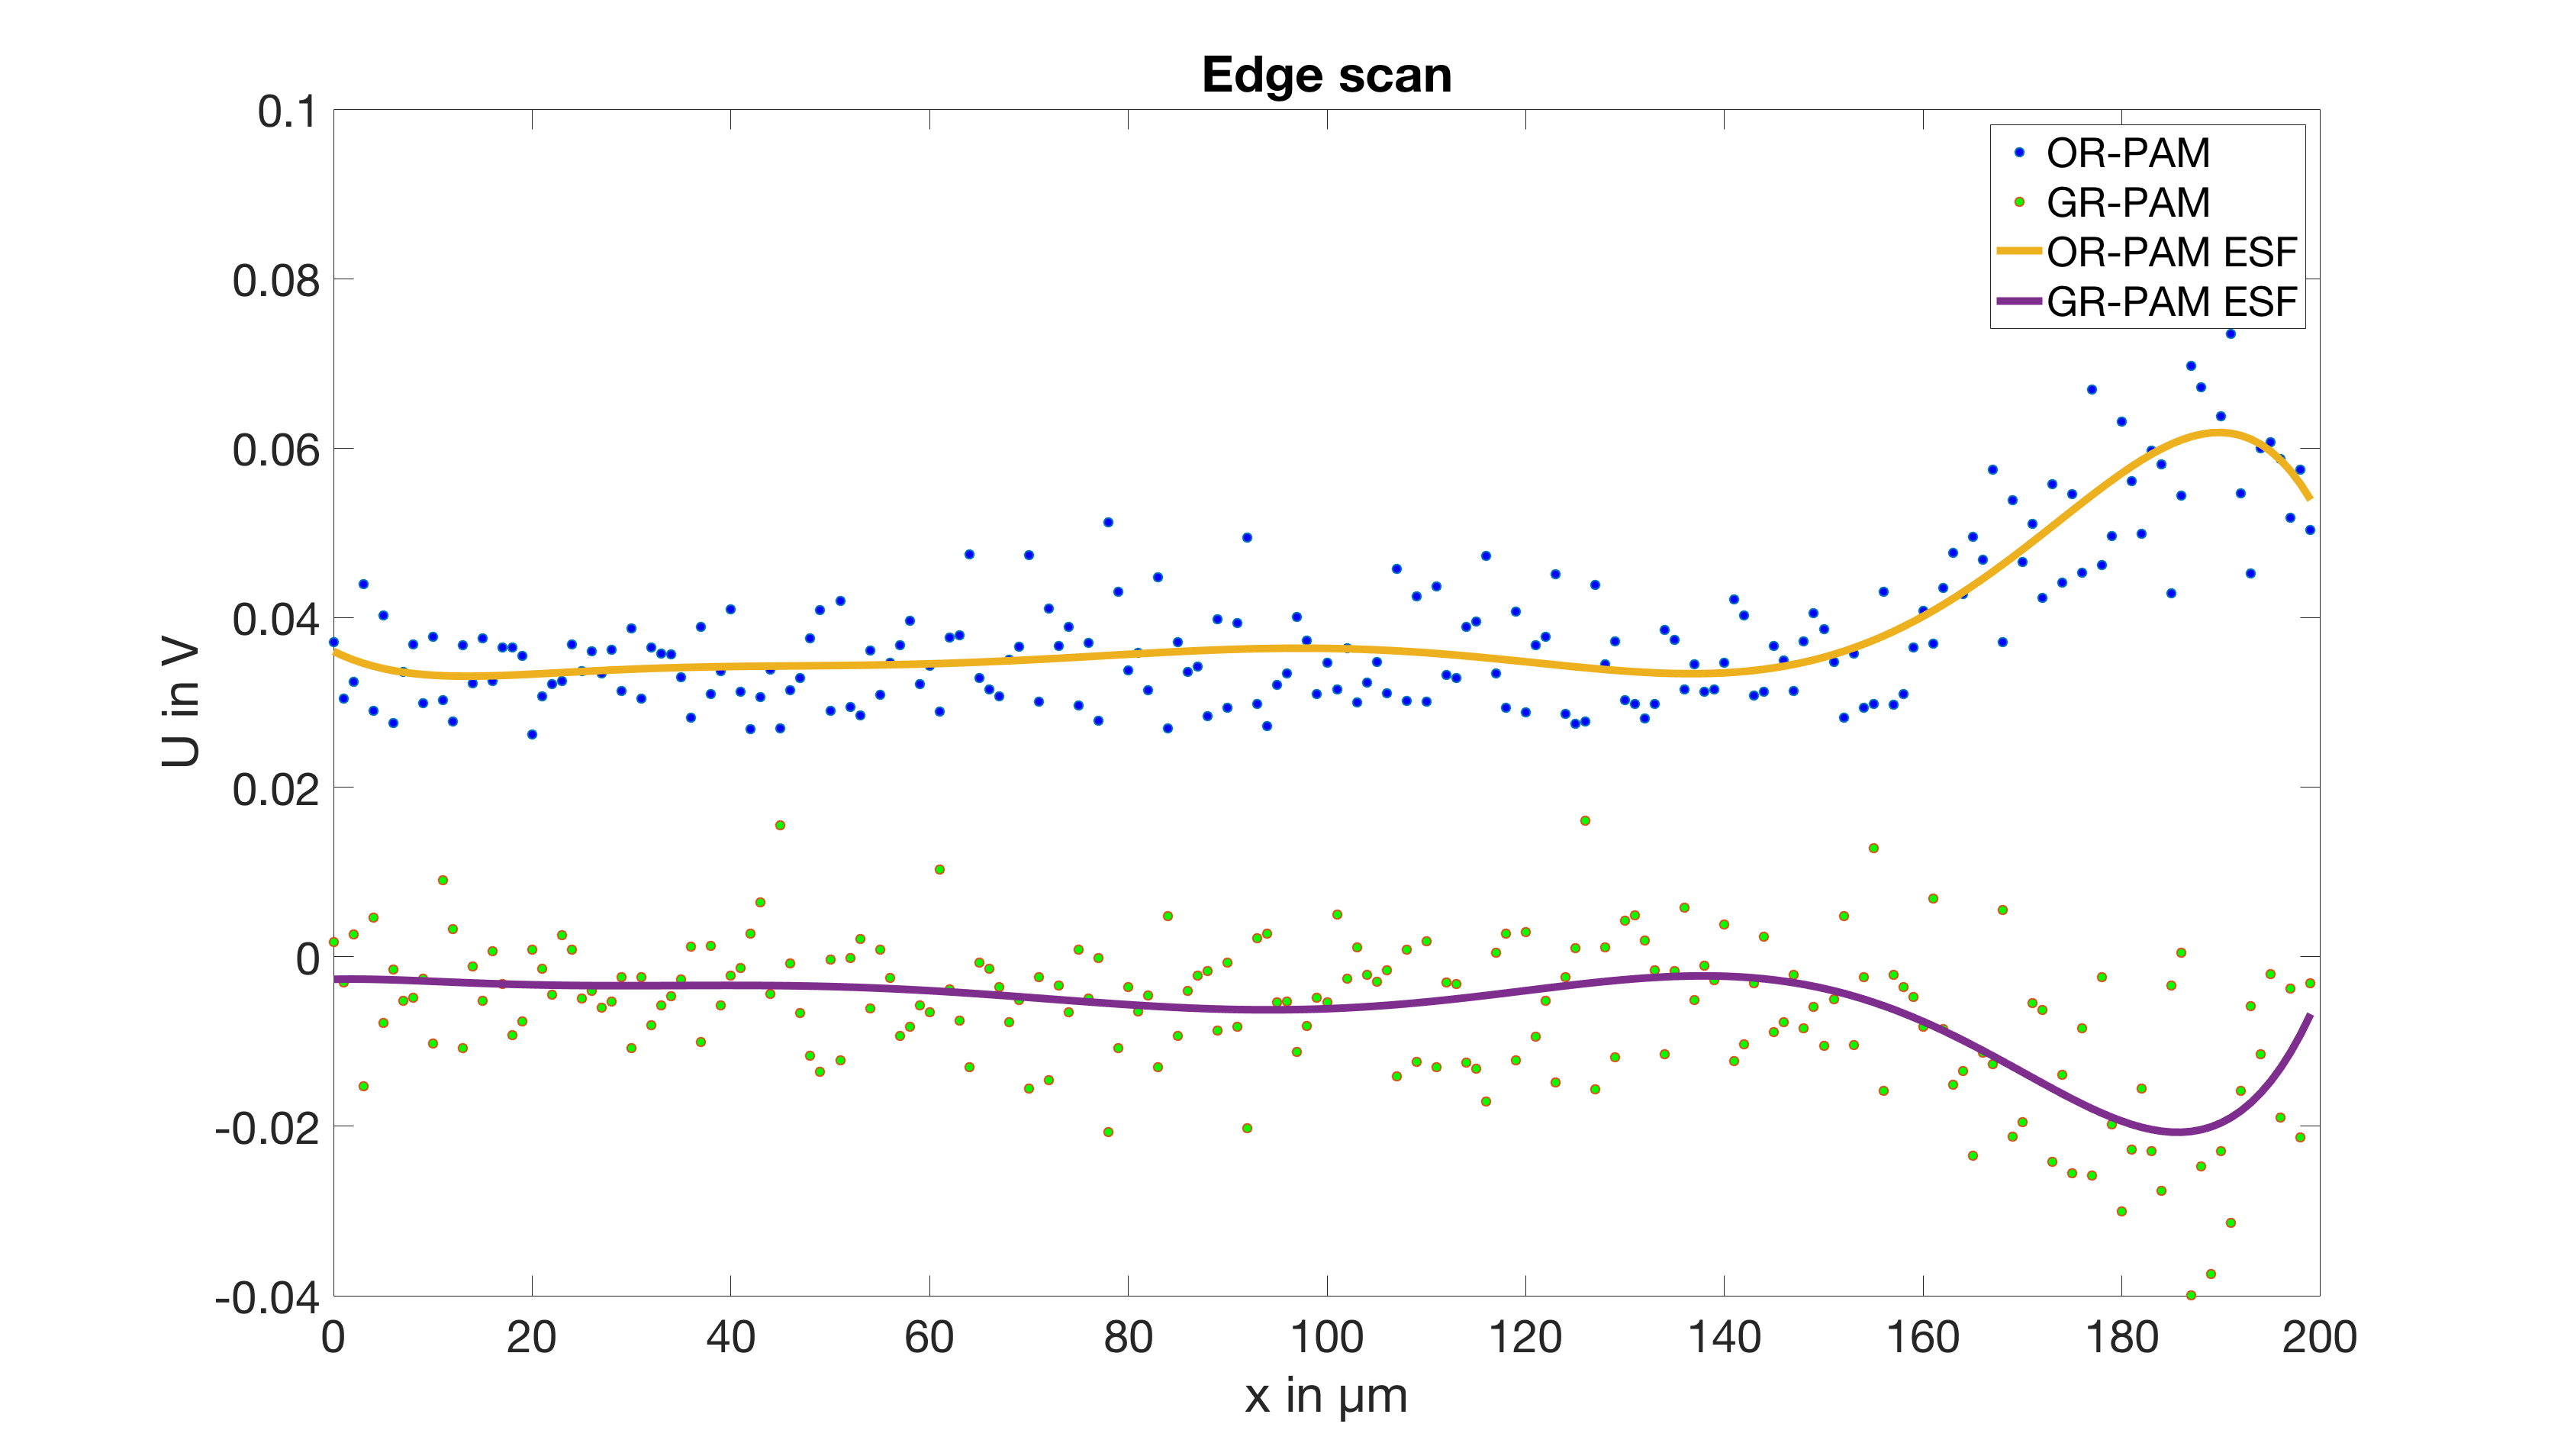
\includegraphics[width = \textwidth, height=0.25\textheight]{04_ex-results_of_PAM/images/ESF.png}
 	\end{minipage}	
 	b)
 	\begin{minipage}{0.5\textwidth}		
 		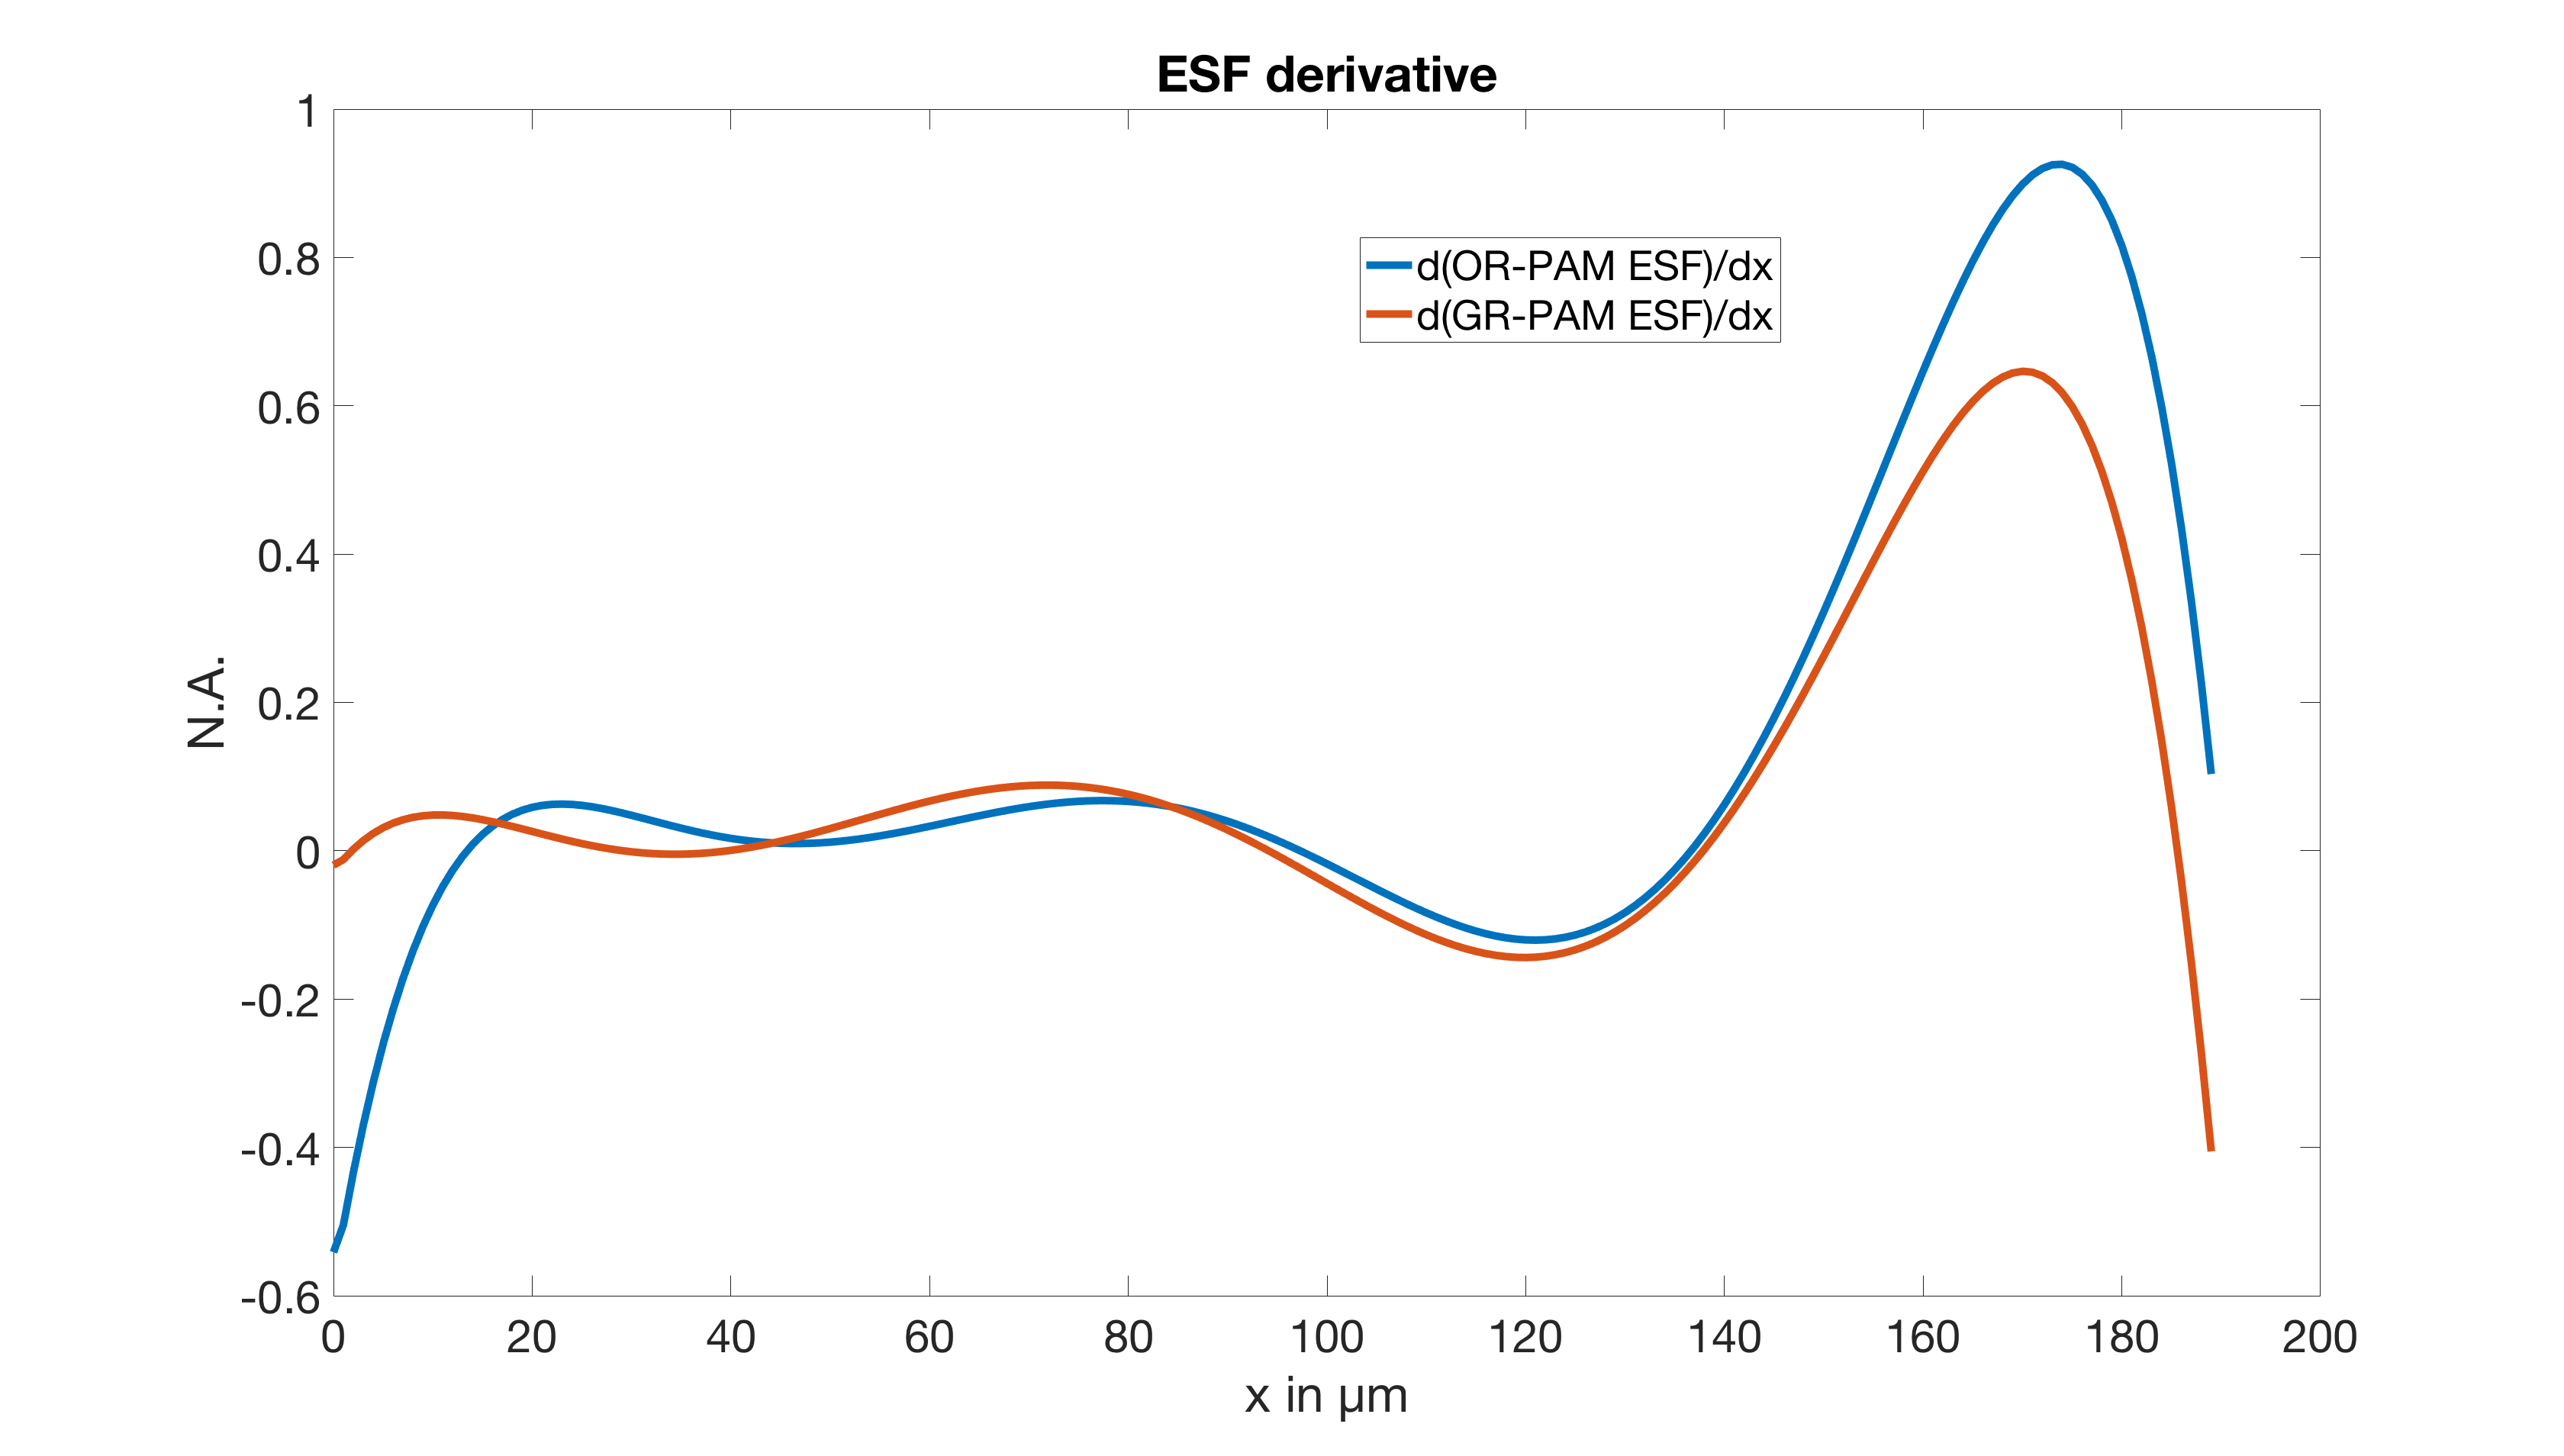
\includegraphics[width = \textwidth, height=0.25\textheight]{04_ex-results_of_PAM/images/ESFderivative.png}
 	\end{minipage}
 	
 	\caption{In a) the measured data points of the scan over an edge are displayed. These are fitted by an polynomial fit of order 9, which is the ESF. Figure b) shows the derivative of the fit function. Here 200 datapoints are taken at a 1$\mu m$ increment.}
 	\label{fig:ESF}
 \end{figure}

Figure \ref{fig:ESF} shows a measurement and analysis of the investigated setup. The FWHM and therefore the resolution of OR-PAM is 31.3$\mu m$ and 29.3$\mu m$ for GR-PAM. Which is an improve of about 7$\%$. The value differs from the 41$\%$ calculated in \ref{sec:resConGR}. \\
A possible explanation for this discrepancy could be, that the change in $\Gamma$ occurs from the surrounding water and not from the resolution target. Because the elements of the resolution target are coated with chromium, which is a good heat conductor. Therefore the applied temperature change is transfered and stored in the water for the acoustic coupling. Furthermore, the chromium layer is very thin and the spherical pressure wave is generated on top of the chromium-water interface. This leads to an interference with the chromium-glass interface reflection.\\
To conclude, there is a measurable resolution improvement in GR-PAM, but the measurement should be done on an edge that contains an absorbing material with low heat conduction. 

\subsubsection{Thermal relaxation time}

The typical delay time between the two GR-PAM pulses in the measurements done before is 60~$\mu s$. The value is determined by trial and error and was completely practicable for the imaging tasks. \\
Therefore it become apparent to investigate in the thermal relaxation time of water, as water is the coupling media and main constituent in the used specimen. \\
In figure \ref{fig:thermalRelaxTime} the amplitude increase due to the Grueneisen effect is displayed in percent over the delaytime between the pulses.

\begin{figure}[H]
	\centering
	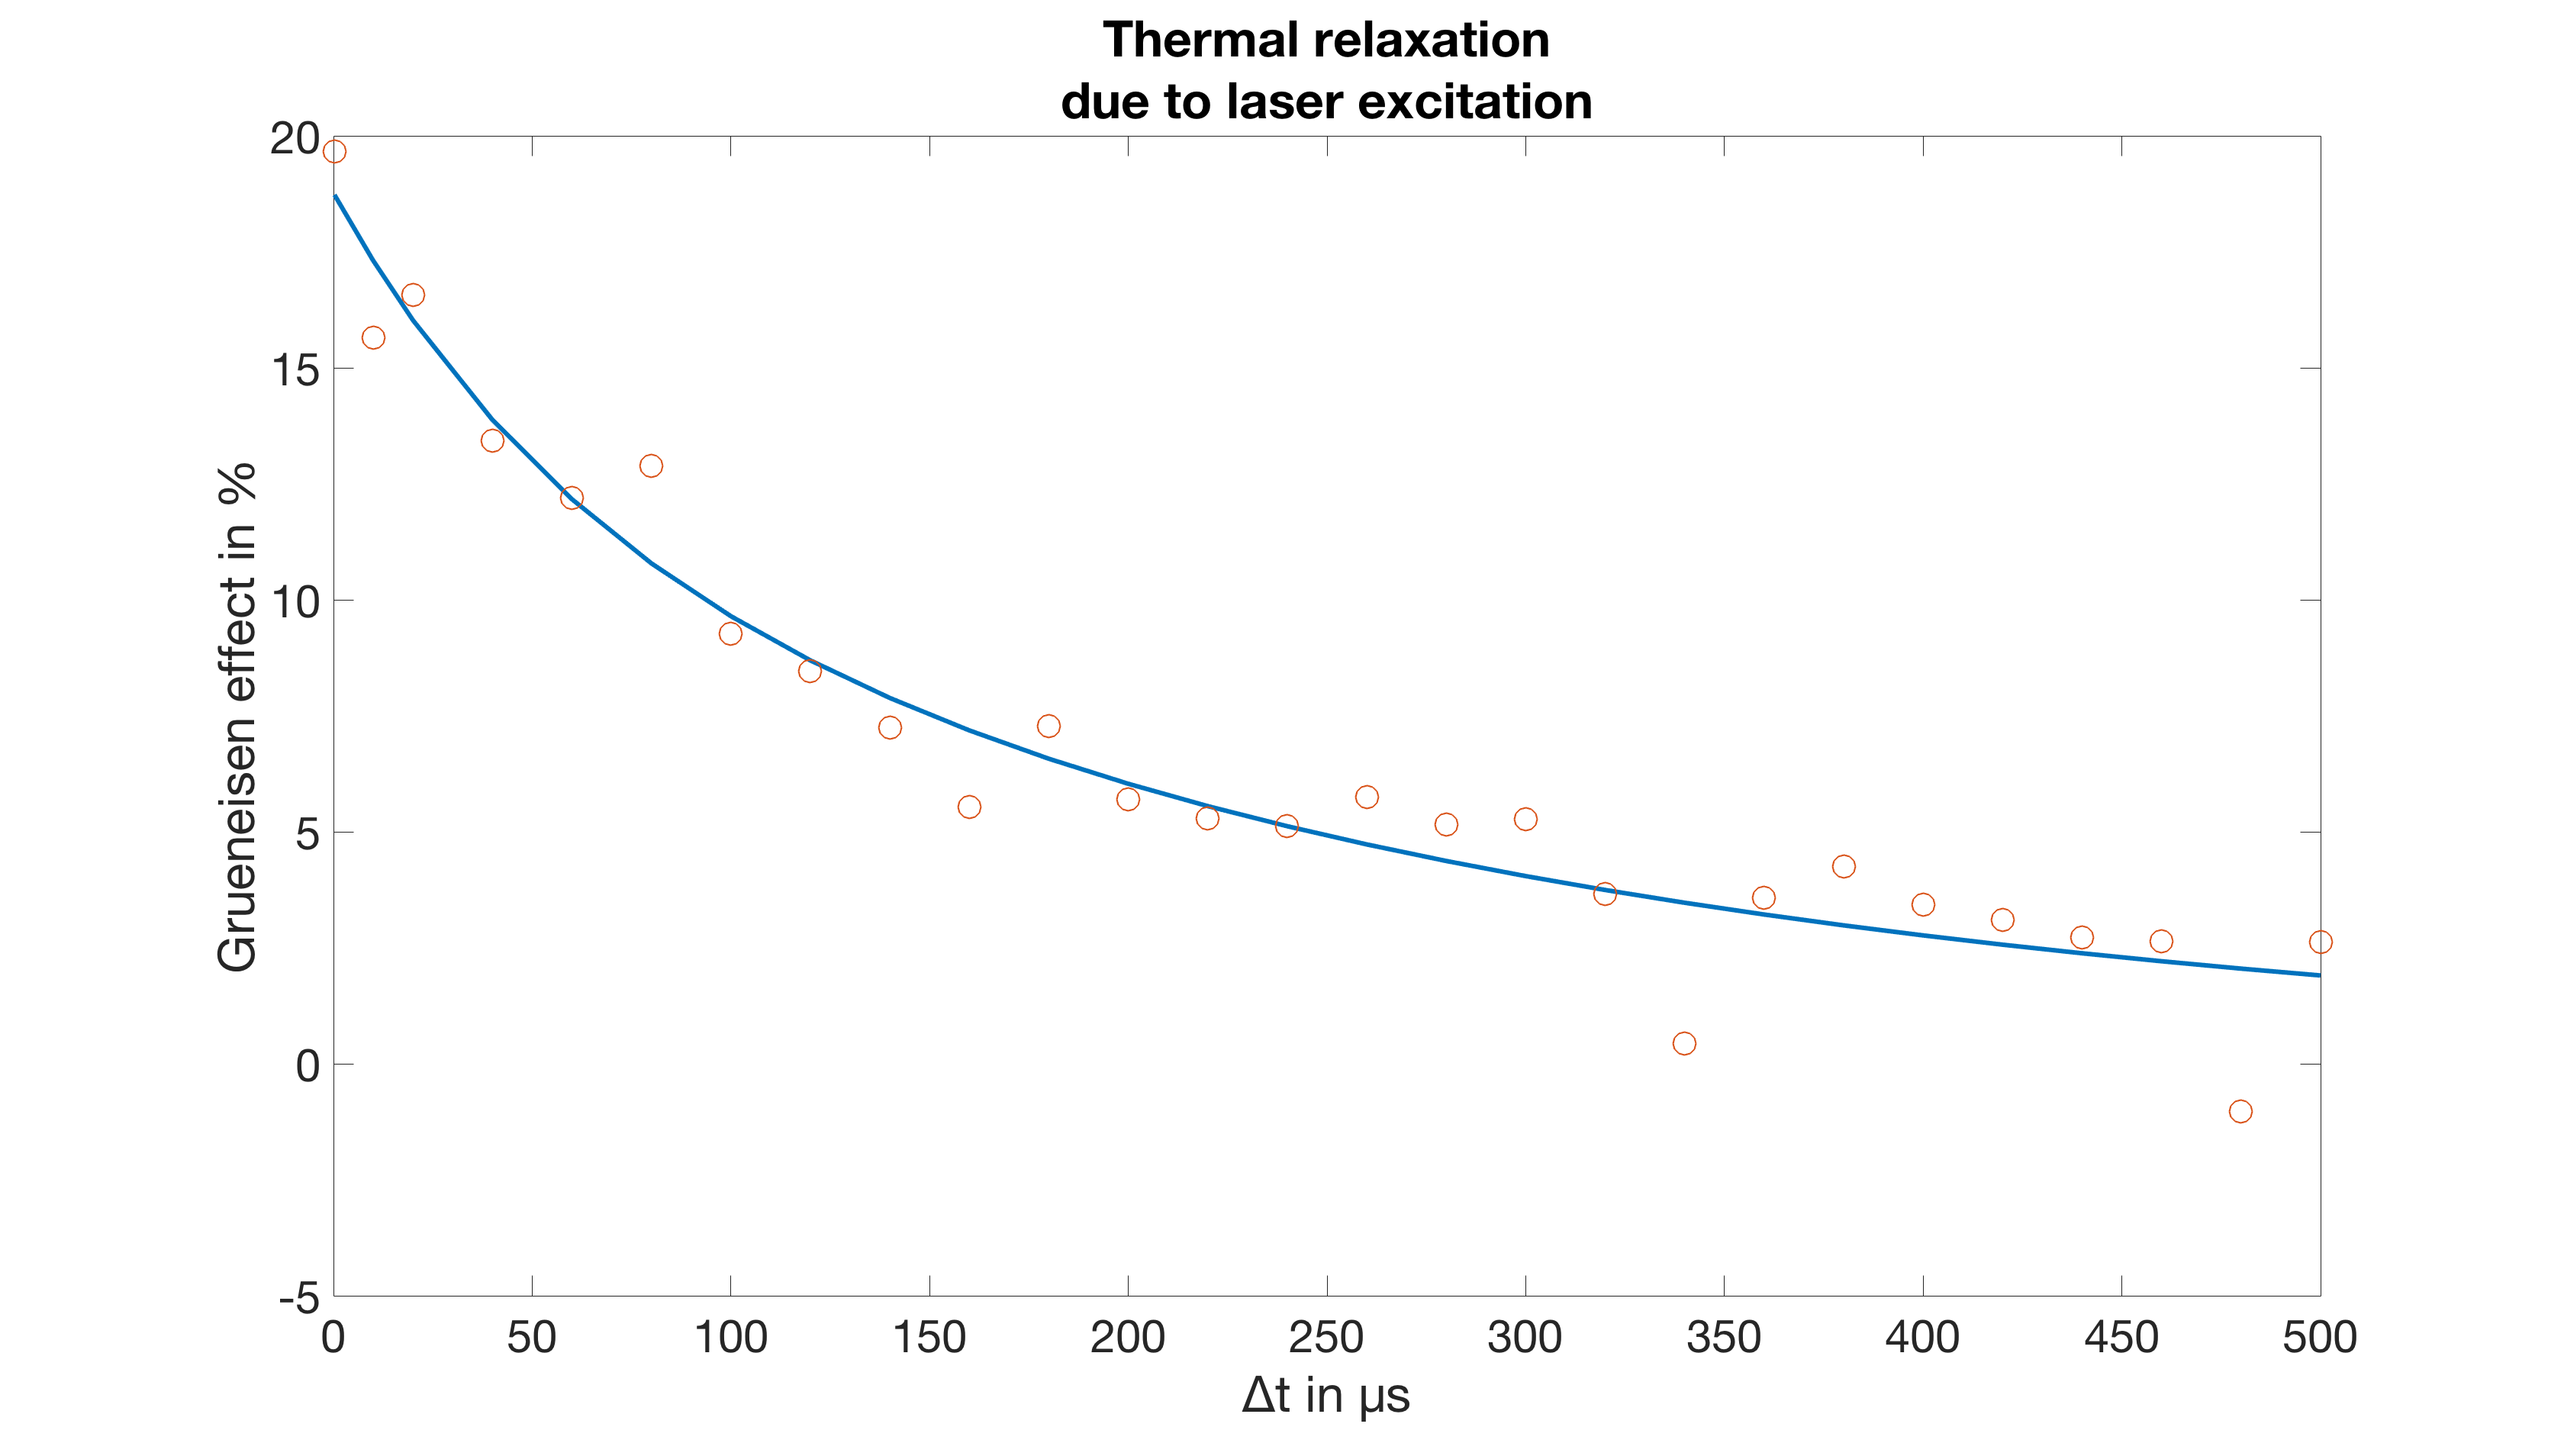
\includegraphics[ height=0.35\textheight]{04_ex-results_of_PAM/images/thermalRelaxTime.png}
	\caption{The dependency of the Grueneisen effect on the delay time between heating and detection laser pulse, for OrangeG colored water. The fitted curve parameter for the relaxation time is $\tau_{water}$ = 270.27~$\mu s$}
	\label{fig:thermalRelaxTime}
\end{figure}

It can be seen that the Grueneisen effect declines as the delay time increases. \\
Also the taken value of 60~$\mu s$ generates in the OrangeG colored water a Grueneisen effect of about 12~$\%$. Therefore the estimated value is suitable for the measurements. 

\subsection{Topographical analysis of OR-PAM images}
\label{sec:topoPAI}

The 3D data cube, described in section \ref{sec:DAQ}, produced by OR-PAM, can be used to map topographical properties.\\
Figure \ref{fig:blackleaf3D} shows a example for such a data volume.

\begin{figure}[H]
	\centering
	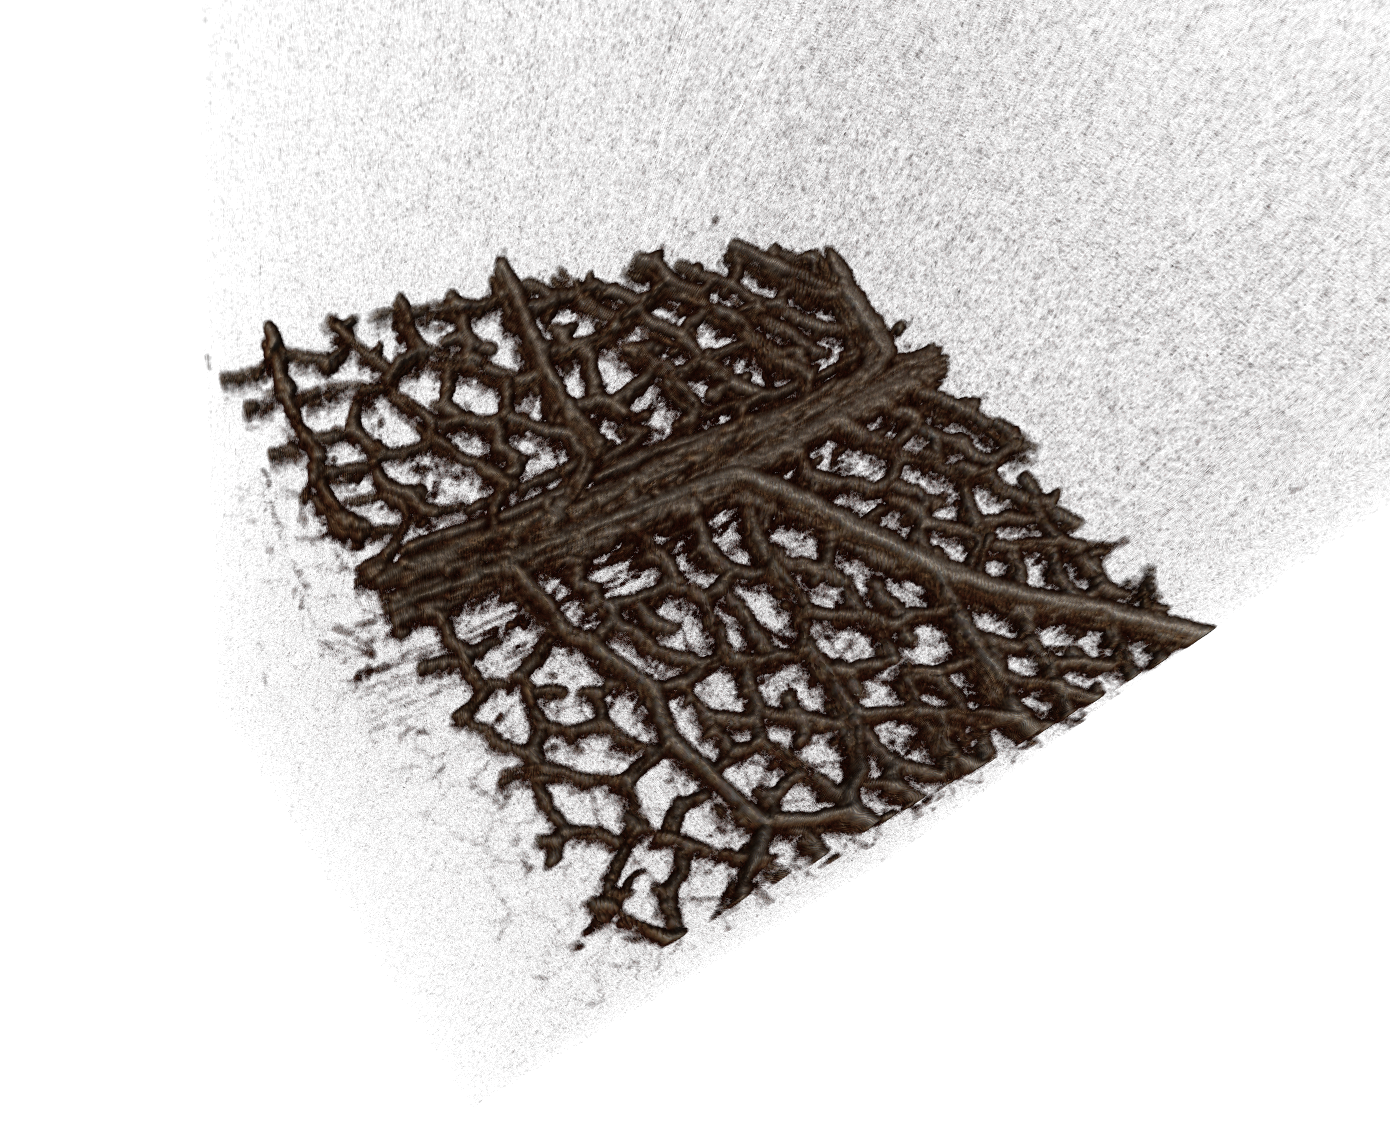
\includegraphics[ height=0.35\textheight]{04_ex-results_of_PAM/images/OR_PAM3G.png}
	\caption{3D image of a black leaf sample. The image size is 8 x 8~$mm$, there the step size is 40~$\mu m$ and 200 steps in each direction.}
	\label{fig:blackleaf3D}
\end{figure}

The sample were a black plastic leaf, which has good absorption properties at the used laser excitation wavelength of 527~$nm$. The dark shadows below the maximum amplitude plane are reflexions from the downside of the leaf and the sample carrier.\\
The structure of the leaf is clearly visible, moreover, the difference in height between the smaller ramification and the main strand. Therefore, the runtime of the ultrasonic waves can be interpreted to gain topographical images of surfaces. This analysis method is applicable to every material where the photoacoustic effect is achievable.\\
Figure \ref{fig:coin3D} shows the 3D image of a coin. 

\begin{figure}[H]
	\centering
		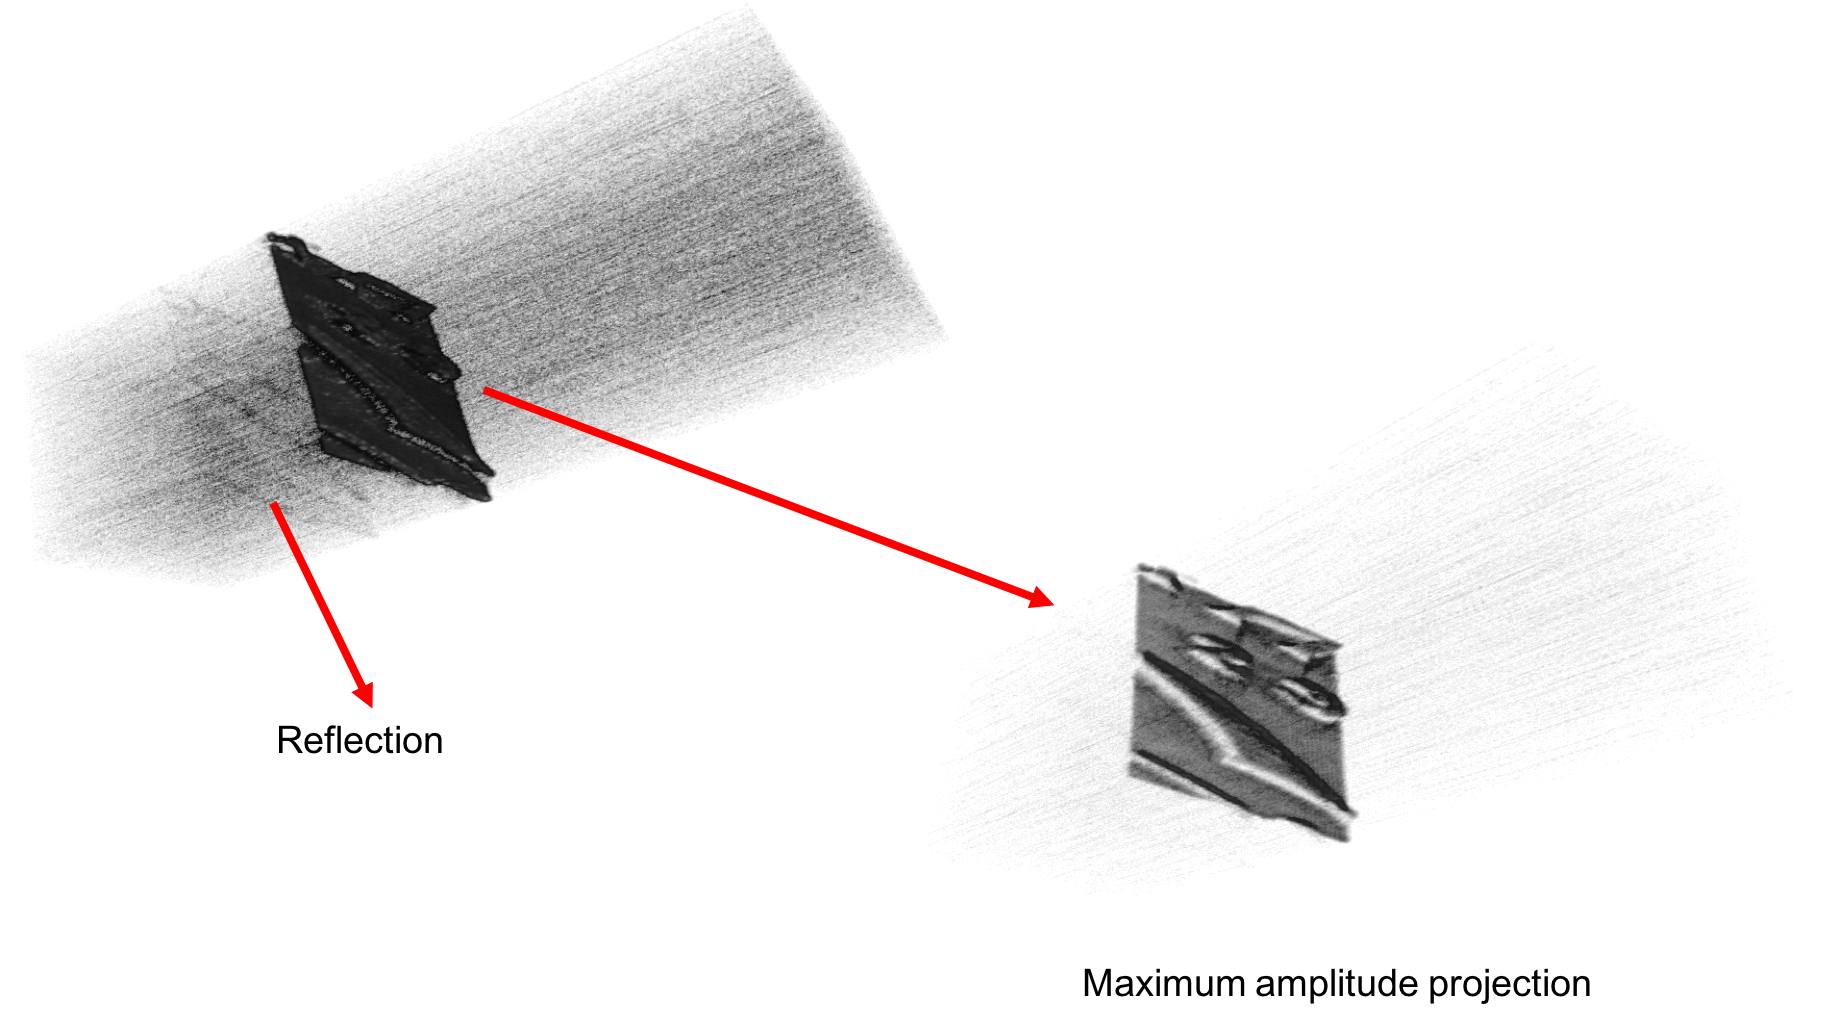
\includegraphics[width = 0.75\textwidth, height=0.28\textheight]{04_ex-results_of_PAM/images/coin3Dzoom.jpg}
	\caption{3D information block of a coin. The image size is 8 x 8~$mm$, there the step size is 40~$\mu m$ and 200 steps in each direction.}
	\label{fig:coin3D}
\end{figure}

Additional to the determination of topographical properties the backside- and other reflections can be used to determine layer thickness of the sample or its quality. \\
Another property that can be determined is the sample tilt in respect to the scan plane. Thus figure \ref{fig:sampletilt} shows the comparison between the maximum amplitude and runtime around a average value, taken from the black leaf data volume shown in figure \ref{fig:blackleaf3D}. The heatmap for the runtime is converted into length scale. 

\begin{figure}[H]
	\centering
	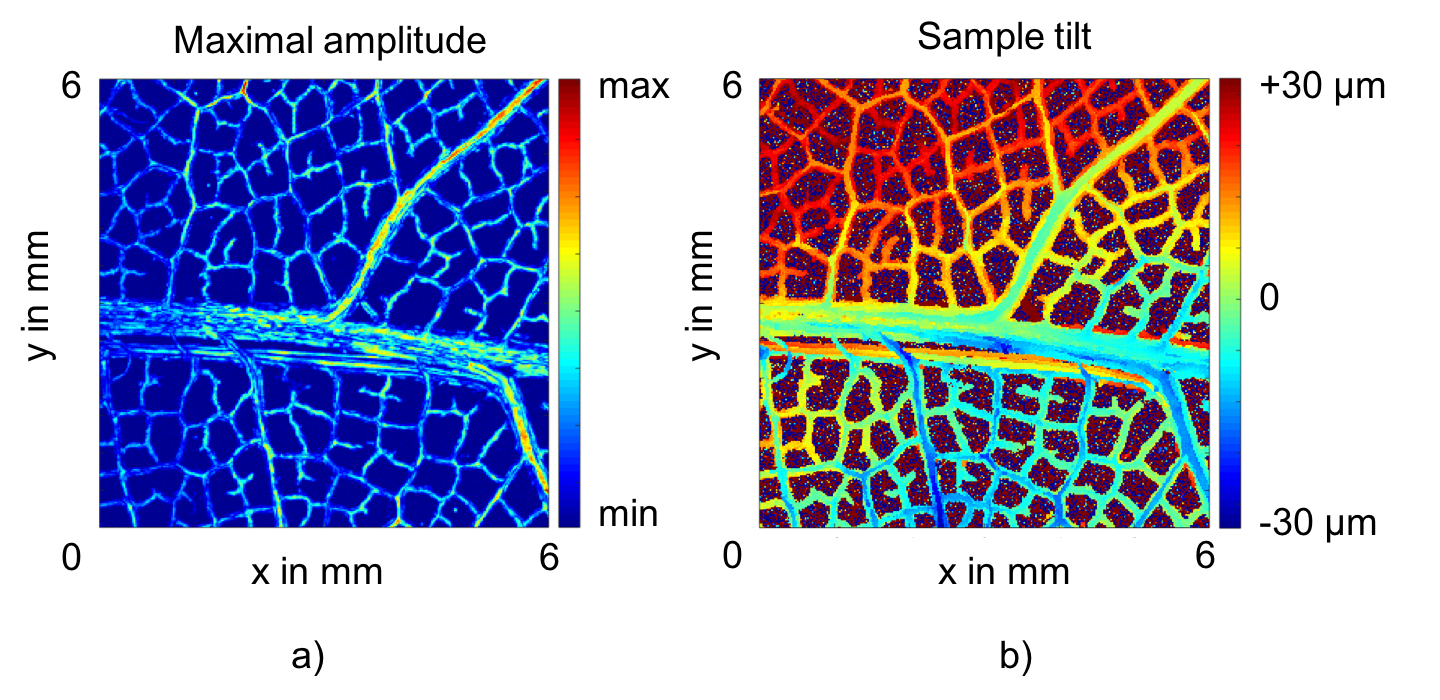
\includegraphics[ width = 0.95\textwidth, height=0.3\textheight]{04_ex-results_of_PAM/images/sampletilt.jpg}
	\caption{In a) the maximum amplitude from the black leaf data set is taken and b) shows a runtime analysis.}
	\label{fig:sampletilt}
\end{figure}

The red shaded area in figure \ref{fig:sampletilt} b) is the part where the ultrasonic signal arrived earlier than in the blue shaded parts. Therefore the upper left corner is closer to the scan plane than the lower right corner. This corresponds to a tilt of the sample. 


